\chapter{Descrizione del modello}
\label{chapter:model}

In questo capitolo verrà descritto in dettaglio il modello del supermercato da noi implementato; in particolare vedremo il framework utilizzato per implementare il modello, le motivazioni che ci hanno portato a costruire un modello ad agenti, gli agenti Cliente e Cassa visti nel particolare, l'ambiente fisico in cui agiscono gli agenti, come essi interagiscono, infine i pattern e i parametri implementati per rendere il modello flessibile.

\section{Framework adottato}
Mesa \cite{mesa} è un framework in Python usato per la modellazione basata su agenti (ABM). Permette di creare il modello con componenti \textit{built-in} come griglie spaziali e scheduler di agenti, e di visualizzare i componenti del modello con un'interfaccia browser. Sfruttando Mesa è possibile definire sia l'ambiente che gli agenti estendendo le relative classi messe a disposizione dal framework. Mesa infine comprende strumenti per l'analisi del modello creato.

Nel nostro modello di supermercato, il modello vero e proprio di Mesa è la classe \textbf{Supermarket} e gli agenti sono i clienti, classe \textbf{Customer}, e le casse, classe \textbf{CashDesk}. 

\section{Sistema}

Il supermercato è stato progettato come \textbf{sistema multi-agente}, comprendente agenti Cliente e Cassa, con l'obiettivo di indagare sulle scelte individuali dei clienti, infatti lo scopo del progetto è trovare la migliore strategia di scelta della coda al fine di minimizzare i tempi d'attesa. La presenza di strategie individuali rende utile la modellazione ad agenti, infatti vorremmo che dai comportamenti dei singoli clienti emergano alcune proprietà del sistema, come la non linearità, che non si possono predire a priori.

La scelta del modello ad agenti è in realtà molto naturale: il supermercato è un sistema complesso in cui diverse entità interagiscono e cercano di risolvere alcuni problemi. I clienti effettuano scelte individuali, hanno obiettivi (la spesa, il tipo di pagamento) e i lavoratori e le casse sono lì per soddisfare i loro bisogni; i clienti e i lavoratori devono interagire per far "evolvere" il sistema supermercato durante la giornata, per raggiungere i loro obiettivi.

Qualunque sistema umano, in particolare che comprenda le decisioni umane, ha una componente impredicibile, stocastica; per questo abbiamo voluto inserire, soprattutto nelle decisioni dei clienti, delle variabili che dipendono da delle distribuzioni di probabilità. Per questo motivo il sistema descritto in questa relazione non è deterministico ed ogni simulazione è diversa dalle altre.

Il sistema supermercato è multi-agente perchè in esso agiscono tanti agenti, in particolare il numero di clienti presenti varia nel tempo, mentre il numero di casse resta costante durante una simulazione. Come si vedrà nelle sezioni \ref{model:customers} e \ref{model:cashdesks}, gli agenti Cliente e gli agenti Cassa sono di tipo diverso (goal-based e model-based reflex, rispettivamente), per cui il supermercato è un sistema \textbf{eterogeneo}.

\section{Agente di tipo Cliente}
\label{model:customers}
I clienti sono gli agenti principali che compongono il modello e interagiscono con l'ambiente per raggiungere l'obiettivo di fare la spesa; per portare a termine questo compito l'agente esegue alcuni macro-step in cui è necessaria anche una fase di pianificazione e valutazione della bontà (\textit{utility function}) della scelta.

Dal punto di vista dell'agente di tipo cliente, la fase più complicata è quella in cui ha raggiunto il target basekt size e deve quindi mettersi in una coda per attendere il suo turno in cassa.
A questo punto il \textbf{goal dell'agente }è essere servito da una cassa nel minor tempo possibile, pur dovendo necessariamente passare per una coda.
Questa fase richiede una pianificazione da parte dell'agente in quanto la coda viene scelta in modo ottimale cercando di minimizzare il tempo passato in coda, ciò avviene basandosi su diverse strategie che saranno descritte nel capitolo \ref{implementation:intro}. Ragionamenti analoghi vengono fatti nel momento in cui l'agente già in coda decide di fare jockeying, ovvero cambiare la coda attuale perchè questa azione porta al raggiungimento del goal.

Da queste considerazioni è possibile classificare l'agente di tipo Cliente come "utility-based", secondo la tassonomia proposta Russel-Norvig \cite{norvig}; l'architettura di un agente "utility-based" è riportata nella figura \ref{fig:utility-based}.

\begin{figure}[H]
	\centering
	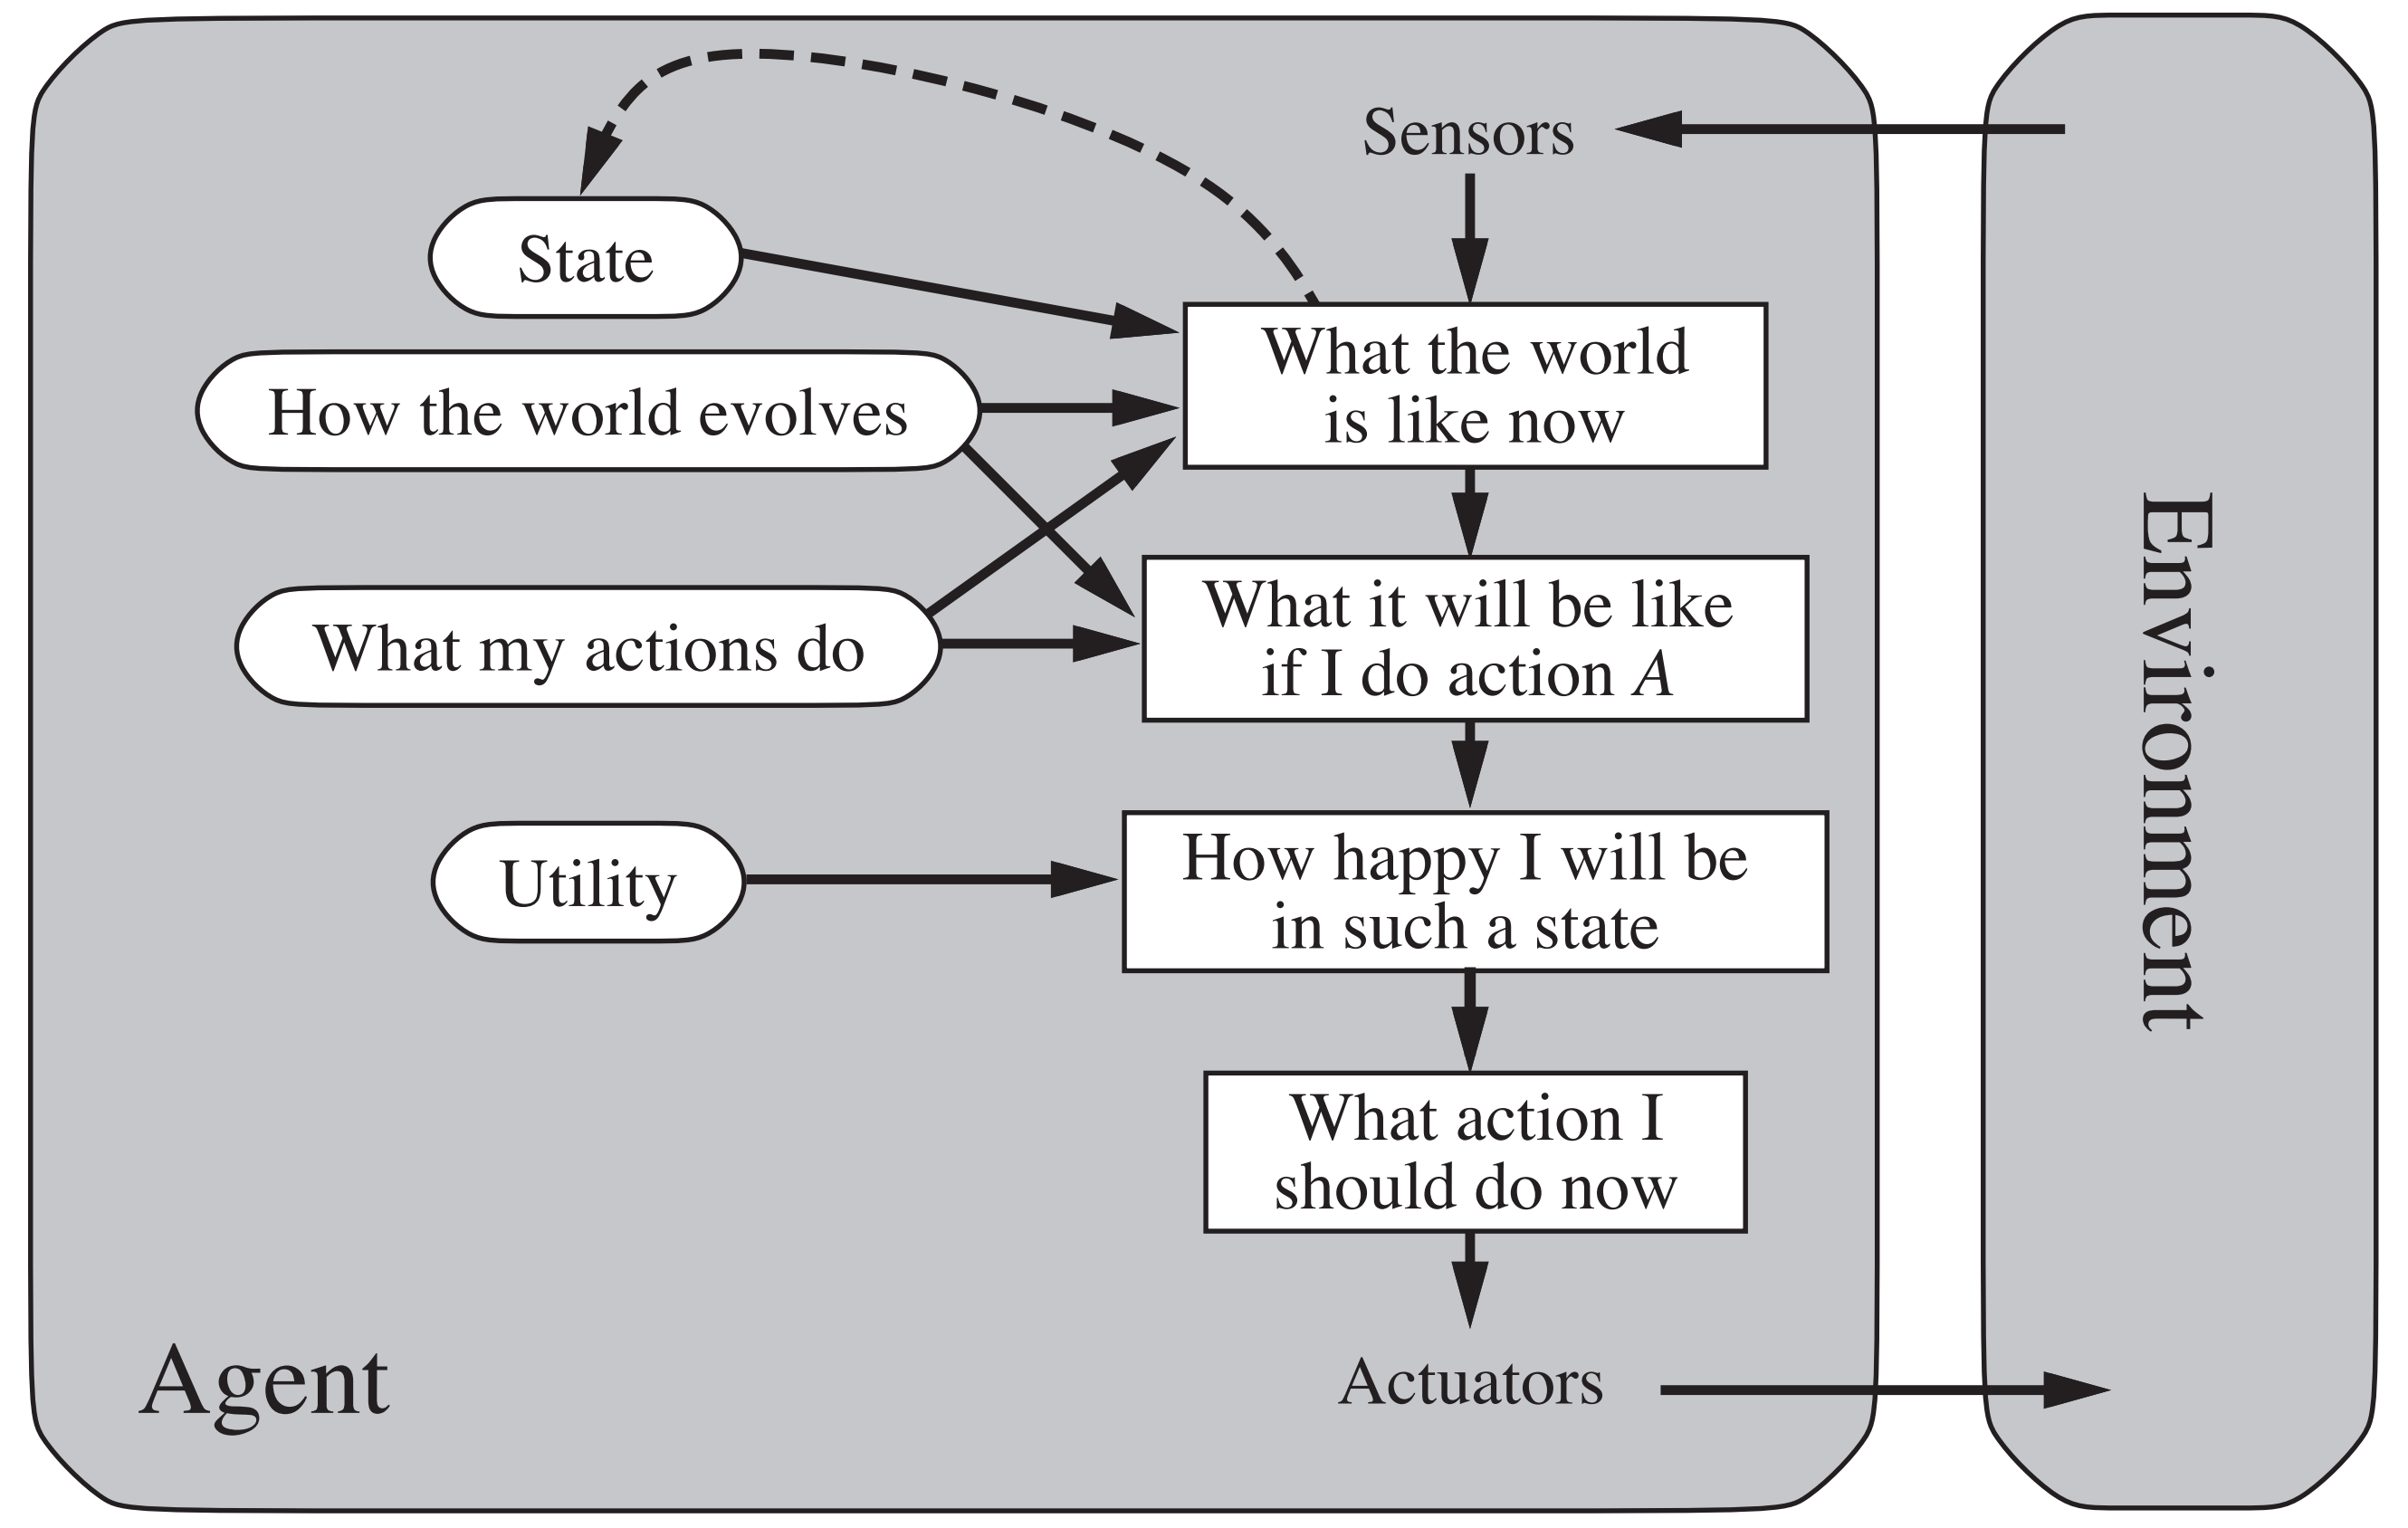
\includegraphics[width=11cm]{"images/utility-based_architecture.png"}
	\caption{Agente di tipo utility-based.}
	\label{fig:utility-based}
\end{figure}

Da questa immagine possiamo notare come ci sia una corrispondenza tra l'architettura proposta e quella dell'agente di tipo cliente. Infatti l'agente pianifica le sue azioni e valuta la bontà dell'azione di scegliere una coda per mezzo di una utlity function.

\subsection{Workflow}
I macro-step che l'agente deve seguire per il raggiungimento del goal, che coincidono con gli stati associati all'agente durante la simulazione, sono:

\begin{enumerate}
	\item \textbf{Attesa all'entrata del supermercato}: in questo stato il cliente si mette in attesa finchè non è possibile entrare nel supermercato.
	\item \textbf{Fase di shopping}: il cliente è entrato e può iniziare a "fare la spesa", con questo si intende raggiungere il numero di prodotti desiderato, infatti nella simulazione viene considerato il \textit{basket size}, un'astrazione del carrello modellato attraverso un numero interno. Il basket size è il target da raggiungere nella fase di shopping, a ogni step il numero di prodotti aumenta di una certa quantità (la velocità di shopping è un parametro del modello descritto nella sezione \ref{model:parameters}). 
	
	La basket size viene generata stocasticamente secondo una distribuzione esponenziale di parametro $\lambda = 0.07361$. La scelta di questo parametro viene giustificata nella sezione \ref{model:parameters}. 
	
	\item \textbf{Scelta della coda}: in questo stato il cliente ha finito di fare la spesa e vuole mettersi in coda ad una cassa. Dal momento che sono disponibili più code e ognuna di queste avrà molto probabilmente altri clienti già in coda, il cliente deve scegliere in quale coda andare in base alla coda che lui considera migliore.
	
	Formalmente viene definita una strategia di scelta della coda in base a una funzione: la \textit{utility function}. Il cliente sceglie quindi la coda $q^*$ che minimizza questa funzione:

	\begin{equation}
		q^* = \operatorname*{argmin}_{q \in Q} f(q) \label{eq:strategy}
	\end{equation}
	dove $Q$ è l'insieme delle code dedicate e $f$ varia a seconda del tipo di strategia che il cliente può utilizzare per la scelta della coda.

	\item \textbf{Attesa in coda e jockeying}: una volta che il cliente ha scelto la coda deve aspettare il proprio turno per essere servito. Nel lavoro di Tomasz Antczak e altri \cite{article1} viene suggerito come sviluppo futuro lo studio del fenomeno di \textit{jockeying}: con questa espressione si intende cambiare la coda che è stata scelta inizialmente in quanto un'altra risulta essere più conveniente, ad esempio perchè più scorrevole.
	
	Ad ogni timestamp l'agente considera le due code adiacenti (parametro spiegato nella sezione \ref{model:parameters} e scelto a priori per il modello) alla propria e per ognuna di queste ricalcola la coda migliore secondo la \ref{eq:strategy}. A questo punto l'agente valuta se per lui è conveniente cambiare la coda o rimanere in quella dove è già presente. Si noti come per effettuare questo confronto è necessario utilizzare l'approccio della \ref{eq:strategy} sulla coda in cui l'agente è in quel momento, andando ad escludere i clienti che si sono inseriti in coda dopo di lui. Una volta fatta questa valutazione, il cliente cambia coda solo se il "guadagno" è maggiore di un certo threshold, anche questo parametro nel modello. A questo punto il cliente può cambiare coda con una certa probabilità, scelta a priori.
	
	La scelta modellistica di effettuare jockeying stocasticamente e in funzione dell'effettivo guadagno di tempo è stata fatta per cercare di avere una rappresentazione il più fedele possibile al mondo reale. Infatti nella realtà un cliente al supermercato potrebbe scegliere di non cambiare la coda nel momento in cui ha un guadagno minimo in quanto questo richiede uno sforzo fisico che non tutti vogliono spendere nella realtà. Inoltre questa operazione richiede che gli agenti controllino continuamente le casse vicine, anche questo non è necessariamente vero in quanto dispendioso di energia. Infatti nel lavoro di Tomasz Antczak e altri \cite{article1} viene fatto notare come questo comportamento non sia molto frequente, tuttavia seppur essendo poco frequente noi lo consideriamo un fattore importante da modellare, adottando le dovute precauzioni e sfruttando la stocasticità dell'azione.
	
	\item \textbf{Attesa alla cassa}: in questa fase il cliente è arrivato alla cassa, essendo arrivato con lo stato precedente in prima posizione della coda. Da questo punto in poi verrà servito dall'agente di tipo cassa che avrà la responsabilità di processare il basket size del cliente. Dal momento che ci sono diversi tipi di casse, questa fase dipende dall'agente di tipo cassa e non dal cliente. Il cliente deve attendere la fine dell'elaborazione della spesa e quindi uscire dal negozio.
\end{enumerate}

Il workflow dell'agente di tipo cliente viene astratto e riassunto da questa immagine:


\begin{figure}[H]
	\centering
	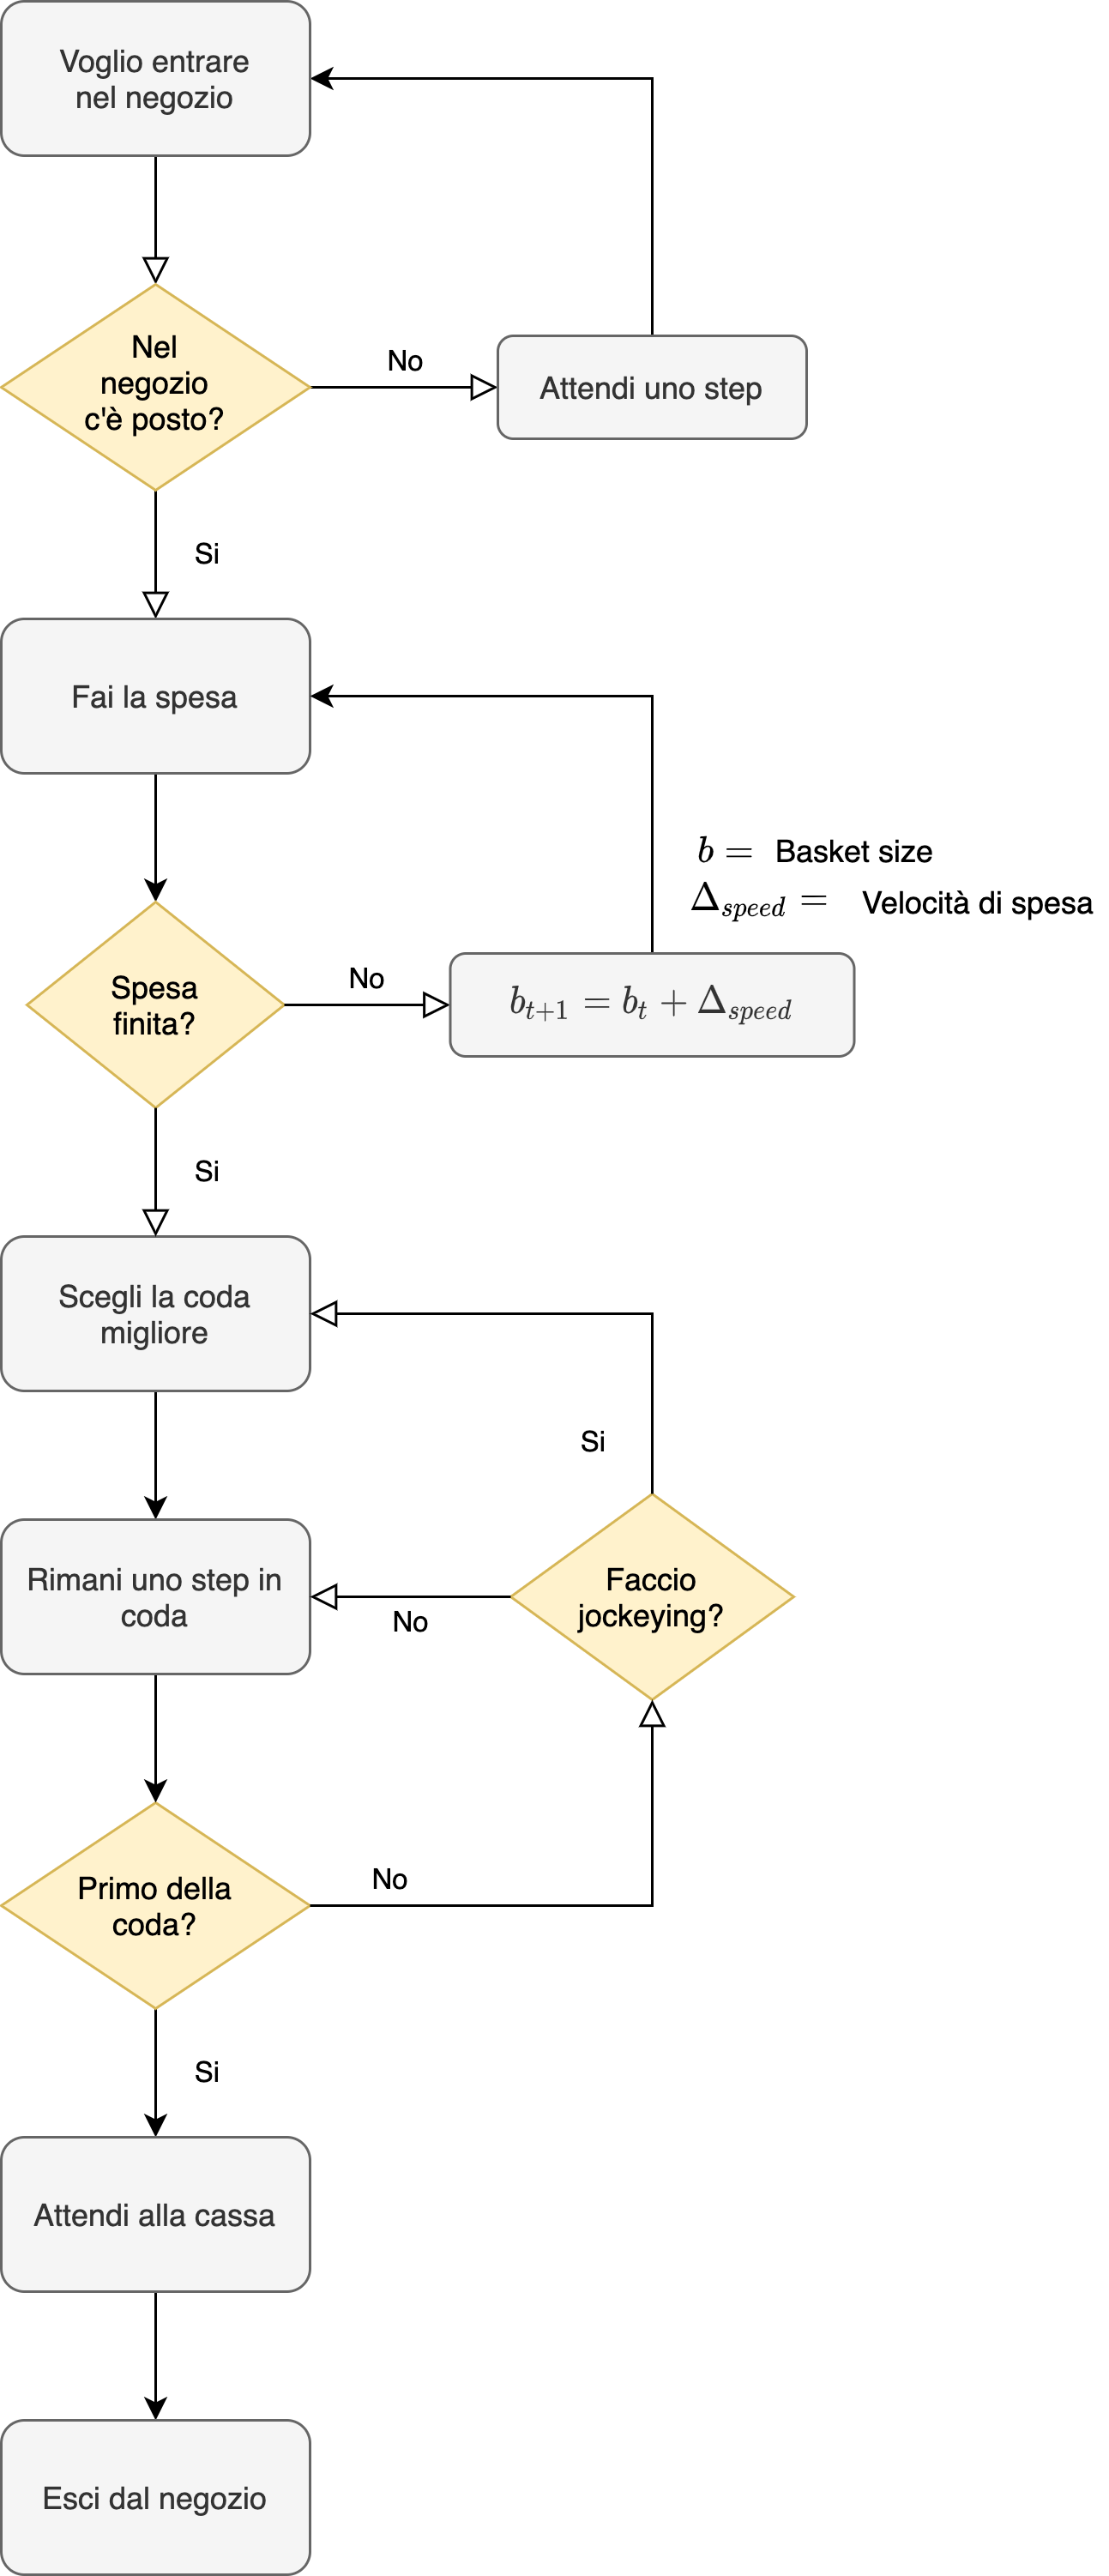
\includegraphics[width=8cm]{"images/workflow_customer.png"}
	\caption{Workflow dell'agente di tipo customer.}
	\label{fig:workflow_customer}
\end{figure}

\section{Agente di tipo Cassa}
\label{model:cashdesks}

Mentre i clienti sono gli agenti principali del sistema supermercato, che si muovono e svolgono le azioni interagendo con esso, le casse sono agenti statici nella griglia della simulazione; le casse non effettuano azioni per se stesse, ma attendono fino a che non ci sono clienti in coda per servirli, e permettergli di effettuare le transazioni di pagamento. Per servire i clienti, la cassa necessita di una rappresentazione del proprio stato, che dipende dalla presenza o meno di clienti e dal loro basket size, di cui ha bisogno per effettuare il pagamento. L'unica decisione individuale che può prendere una cassa, e questo vale soltanto per le casse di tipo standard che si vedranno più avanti, è la propria attivazione o disattivazione in base al numero di clienti presenti nel negozio; l'essere attiva o disattiva fa parte dello stato interno della cassa.

Poichè la cassa non ha obiettivi ma solo il compito di attivarsi e servire gli eventuali clienti in coda, può essere classificata come "model-based reflex agent" secondo \cite{norvig}, descritto in figura \ref{fig:model-based}.

\begin{figure}[htp!]
	\centering
	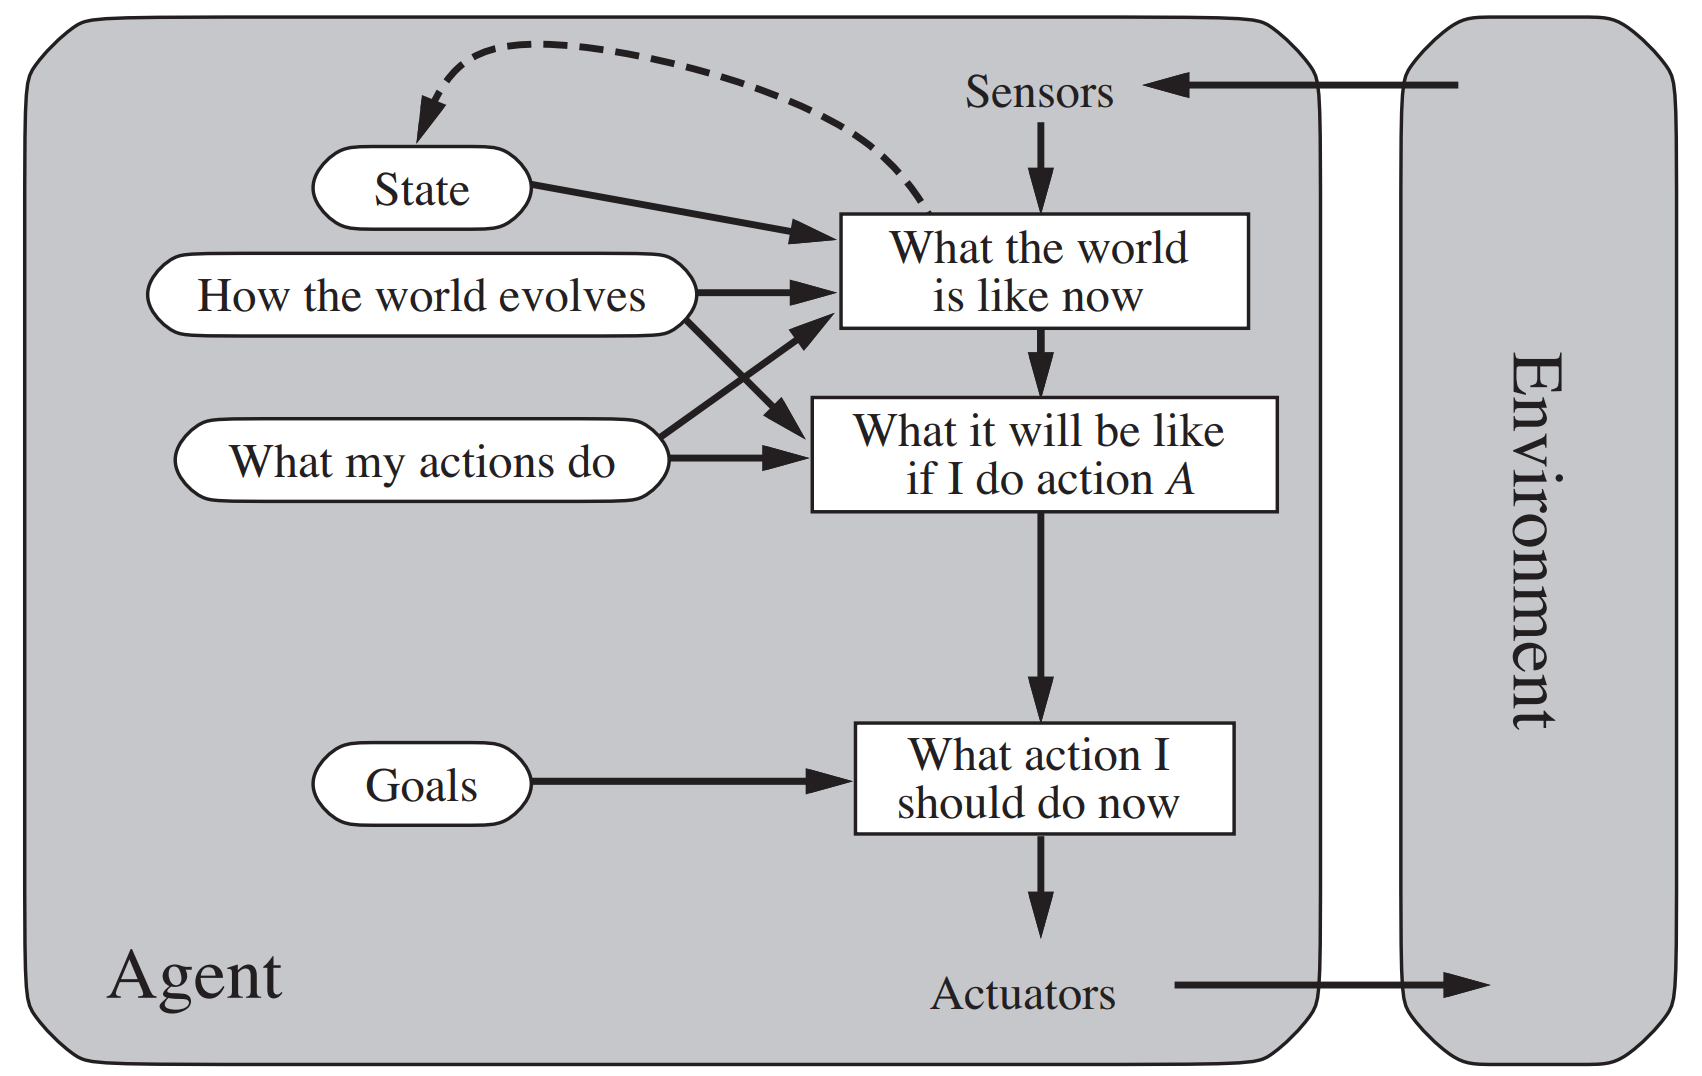
\includegraphics[width=11cm]{"images/model-based-reflex_architecture.png"}
	\caption{Agente di tipo model-based reflex.}
	\label{fig:model-based}
\end{figure}

\subsection{Tipi di cassa}
\label{sec:tipi_cassa}

Gli agenti di tipo cassa hanno l'unica funzione di servire i clienti che si mettono in coda per pagare la spesa; sono di 4 tipi e differiscono per modalità di elaborazione della spesa del cliente e per velocità.

\begin{enumerate}
\item \textbf{Cassa standard}: questa cassa rappresenta la normale cassa che si trova solitamente in tutti i supermercati, all'interno della quale lavora un cassiere che si occupa di passare i prodotti del carrello del cliente sul nastro.
 
Il tempo di servizio di un cliente per questo tipo di cassa è formato da due tempi diversi: il \textbf{transaction-time}, che è il tempo vero e proprio durante il quale avviene la transazione, e il \textbf{break-time}, che è il tempo che passa tra il servizio di un cliente e di un altro ed include anche la fase in cui il cliente insacchetta i prodotti acquistati. Il transaction-time è stato stimato con una regressione di potenza e il break-time con una distribuzione Gamma. In particolare, per un cliente in coda $c_i \in q$, i due tempi sono calcolati in questo modo:

\begin{equation}\label{eq:transaction-time-standard}
\text{transaction-time}_i = e^{a log(\text{basket-size}(c_i)) + b}
\end{equation}
\begin{equation}\label{eq:break-time-standard}
\text{break-time}_i = \frac{\beta^{\alpha} \text{basket-size}(c_i)^{\alpha - 1} e^{- \beta \text{estimate-basket-size}(c_i)}}{\Gamma (\alpha)}
\end{equation}

Dove $\Gamma$ è la funzione \textbf{gamma} e corrisponde a:

\begin{equation}
\Gamma (z) = \int_{0}^{\infty} x^{z-1} e^{-x} dx \;\; \forall z \in \mathbb{C}
\end{equation}

Queste stime sono state prese dall'articolo \cite{article1} e in particolare i parametri $a,b,\alpha ,\beta \in \mathbb{R}$ sono:

\begin{equation}
a = 0.6984, \;\; b = 2.1219, \;\; \alpha = 3.074209, \;\; \beta = \frac{1}{4.830613}
\end{equation}

\item \textbf{Cassa self-service}: alla cassa self-service il cliente provvede da solo al passaggio dei prodotti del carrello allo scanner, per cui non è presente un cassiere. Si suppone che il cliente non sia veloce quanto un cassiere esperto a passare i prodotti sullo scanner, per questo la velocità di processing per questa cassa è stata divisa per un fattore $1.5$, uno dei parametri descritti nella sezione \ref{model:parameters}. A causa della velocità ridotta, di solito nei supermercati è posto un limite di \textit{basket size} per accedere alla cassa self-service; nel nostro modello questo limite è posto a 15, per cui se un cliente ha più di 15 elementi nel carrello e non va nel self-scan, deve per forza andare alla cassa standard.

Anche in questo caso il tempo di servizio è diviso in transaction-time e break-time, solo che, a differenza della cassa normale, il break-time risulta più lungo in quanto il cliente inizia ad insacchettare solamente dopo aver passato i prodotti allo scanner, invece nella cassa standard può iniziare già mentre il cassiere passa i prodotti. In questo caso, dunque, il transaction-time e il break-time sono stati stimati entrambi con una regressione di potenza:

\begin{equation}\label{eq:transaction-time-self-service}
\text{transaction-time}_i = e^{a log(\text{basket-size}(c_i)) + b}
\end{equation}
\begin{equation}\label{eq:break-time-self-service}
\text{break-time}_i = e^{c log(\text{basket-size}(c_i)) + d}
\end{equation}

I parametri in questo caso sono:

\begin{equation}
a = 0.6725, \;\; b = 3.1223, \;\; c = 0.2251, \;\; d = 3.5167
\end{equation}

\item \textbf{Cassa self-scan}: la cassa self-scan si differenzia totalmente dalle prime due descritte, il cliente che voglia utilizzarla infatti, deve deciderlo già al momento dell'entrata nel supermercato, in quanto deve scannerizzare i prodotti man mano che fa la spesa e necessita dunque di una macchinetta scanner; una volta arrivato alla cassa self-scan, egli deve semplicemente effettuare il pagamento, saltando quindi le fasi di scanner e insacchettamento che caratterizzano le casse standard e self-service. La velocità di elaborazione della spesa in questo caso è praticamente nulla, in particolare un cliente che inizia il pagamento a una cassa self-scan, lo termina allo step successivo; il tempo di pausa per questa cassa è ugualmente nullo, dato che un cliente paga ed entra immediatamente nella fase di uscita dal negozio.

Chiaramente per evitare che vengano rubati prodotti, i supermercati decidono di effettuare dei controlli random sui clienti che scelgono di usare le casse self-scan. A questo scopo è stata implementata la cassa di tipo riservato.
\item \textbf{Cassa riservata}: questa cassa è identica nel funzionamento a una cassa standard, ciò che cambia è che è riservata alla rilettura della spesa dei clienti self-scan, che avviene in maniera random. Nel momento in cui un cliente si approccia ad una cassa self-scan, viene estratto un numero che determina la \textbf{rilettura parziale} o la \textbf{rilettura totale} della sua spesa;
la rilettura parziale consiste nell'estrazione di 10 prodotti dal carrello e nella verifica che essi appartengano alla lista contenuta nello scanner del cliente, invece la rilettura totale consiste appunto nella rilettura completa della spesa di esso. Le probabilità di rilettura sono parametri del modello ed attualmente corrispondono allo $7.5 \%$ per la rilettura parziale e allo $2.5 \%$ per la rilettura totale.

Il funzionamento e i tempi di servizio sono esattamente gli stessi della cassa standard, considerando un basket size completo per la rilettura totale e un basket size di soli 10 elementi per la rilettura parziale.
\end{enumerate}

Tutti i tipi di cassa attraversano 3 fasi: fase di attesa di un nuovo cliente, fase di elaborazione della spesa del cliente, fase di completamento della transazione.

\paragraph{Code}
Nel modello, per quanto riguarda le sole casse standard, vengono considerati i casi di:

\begin{itemize}
\item \textbf{Code parallele}: per questa disposizione ad ogni cassa è
  associata una coda. Nel momento in cui la cassa è libera il cliente in
  cima alla coda viene spostato alla cassa per procedere con la fase
  di elaborazione della spesa.
\item \textbf{Coda condivisa}: nota anche come \textit{N-fork} in \cite{yanagisawa2011methods}, più casse condividono la stessa coda, nel momento che una qualsiasi delle casse risulta libera il cliente in posizione utile procede alla cassa. Utilizzando questa disposizione non viene ammesso jockeying.
\end{itemize}

\begin{figure}[H]
\centering
\begin{subfigure}{.5\textwidth}
  \centering
  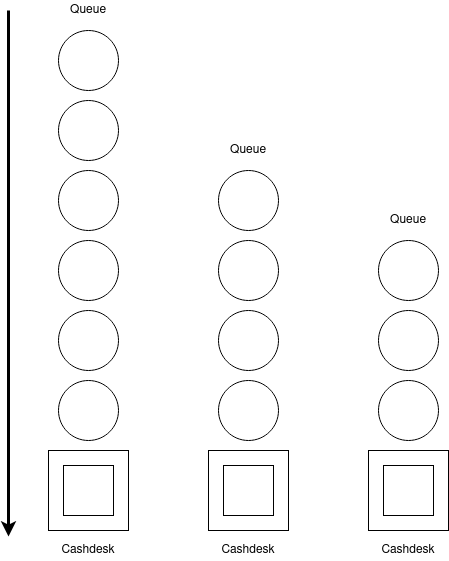
\includegraphics[width=.5\linewidth]{"images/parallel-queues.png"}
  \caption{Code parallele}
  \label{fig:sub1}
\end{subfigure}%
\begin{subfigure}{.5\textwidth}
  \centering
  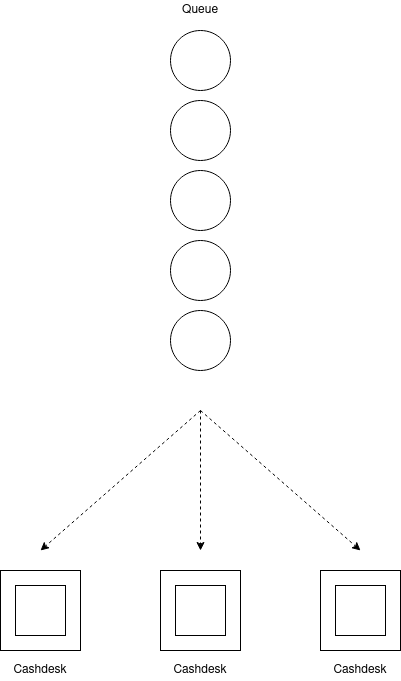
\includegraphics[width=.5\linewidth]{"images/n-fork.png"}
  \caption{Coda condivisa}
  \label{fig:sub2}
\end{subfigure}
\caption{Tipi di code}
\label{fig:test}
\end{figure}


\subsection{Workflow}

\paragraph{Cassa standard}
All'inizio della simulazione, e in generale quando la cassa ha terminato la transazione di un cliente o quando non ci sono clienti in coda, la cassa si trova nella \textbf{fase di attesa di un nuovo cliente}. L'agente cassa chiede alla coda (sia nel caso di code parallele sia nel caso di N-fork) a cui è associata il primo cliente in fila, se ce n'è, quindi compie 4 passi:
\begin{enumerate}
\item Cambia lo stato al cliente che sta servendo, impostandolo in fase di attesa alla cassa
\item Muove il cliente di fianco alla propria postazione, spostandolo quindi dalla coda
\item Cambia il proprio stato impostandolo in fase di elaborazione
\item Fa avanzare tutti i clienti che erano in coda dopo il cliente che viene servito
\end{enumerate}

Nella \textbf{fase di elaborazione della spesa del cliente}, la cassa simula il passaggio dei prodotti sullo scanner, diminuendo il \textit{basket size} del cliente ad ogni passo di una quantità che dipende dalla velocità di processing, parametro del modello. Quando la transazione è completata, ovvero quando il \textit{basket size} del cliente è nullo, fa uscire il cliente dal negozio e cambia il proprio stato, entrando nella \textbf{fase di completamento della transazione}.

In questa ultima fase la cassa ha terminato il servizio di un cliente, quindi si rimette nel primo stato, in fase di attesa di un nuovo cliente.

Il workflow della cassa standard viene riassunto nell'immagine \ref{fig:workflow_cashdesk_standard}.

\begin{figure}[H]
	\centering
	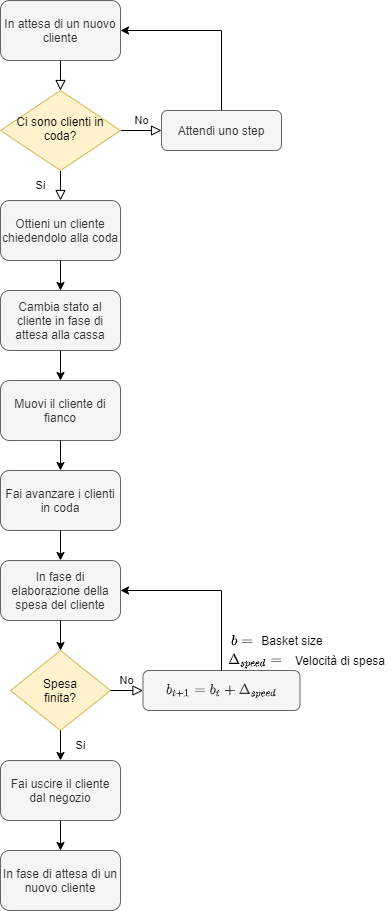
\includegraphics[width=8cm]{"images/workflow_cashdesk_standard.png"}
	\caption{Workflow dell'agente di tipo cassa standard.}
	\label{fig:workflow_cashdesk_standard}
\end{figure}

\paragraph{Cassa self-service}

Il workflow della cassa self-service è uguale in tutto a quello della cassa standard, le uniche differenze sono che esiste una coda condivisa ogni 8 casse self-service (che però funziona allo stesso modo della coda della cassa standard) e che la velocità di elaborazione della spesa è più piccola di 1.5, un parametro del modello.

\paragraph{Cassa self-scan}

Le casse self-scan hanno sempre una coda condivisa, come si può notare in tutti i negozi che hanno adottato questo tipo di cassa. Nella \textbf{fase di attesa di un nuovo cliente}, se ci sono clienti nella coda condivisa, la cassa self-scan prende il primo cliente della coda; estrae quindi un numero e, con il $7.5 \%$ di probabilità lo manda alla cassa riservata per una \textbf{rilettura parziale}, con il $2.5 \%$ di probabilità lo manda alla cassa riservata per una \textbf{rilettura totale} e invece con il $90 \%$ di probabilità gli fa fare il pagamento normale. Nel caso di rilettura parziale o totale, la cassa sposta il cliente alla cassa riservata, fa avanzare i clienti in coda e rimane nella fase di attesa di un nuovo cliente, pronta per prendere il nuovo cliente della coda.

Nel caso non debba avvenire una rilettura la cassa compie queste 4 azioni:

\begin{itemize}
\item Cambia lo stato al cliente che sta servendo, impostandolo in fase di attesa alla cassa
\item Muove il cliente di fianco alla propria postazione, spostandolo quindi dalla coda
\item Cambia il proprio stato impostandolo in fase di elaborazione
\item Fa avanzare tutti i clienti che erano in coda dopo il cliente che viene servito
\end{itemize}

Nella \textbf{fase di elaborazione della spesa del cliente}, la cassa effettua la vera e propria transazione, la differenza con la cassa standard è la velocità di elaborazione della spesa, che in questo caso è uguale alla \textit{basket size} del cliente; il cliente infatti deve soltanto pagare, in quanto ha già scannerizzato i prodotti durante la sua spesa.

Nell'ultima fase la cassa ha terminato il servizio di un cliente, quindi si rimette nel primo stato, in fase di attesa di un nuovo cliente.

Il workflow della cassa self-scan viene riassunto nell'immagine \ref{fig:workflow_cashdesk_self_scan}.

\begin{figure}[H]
	\centering
	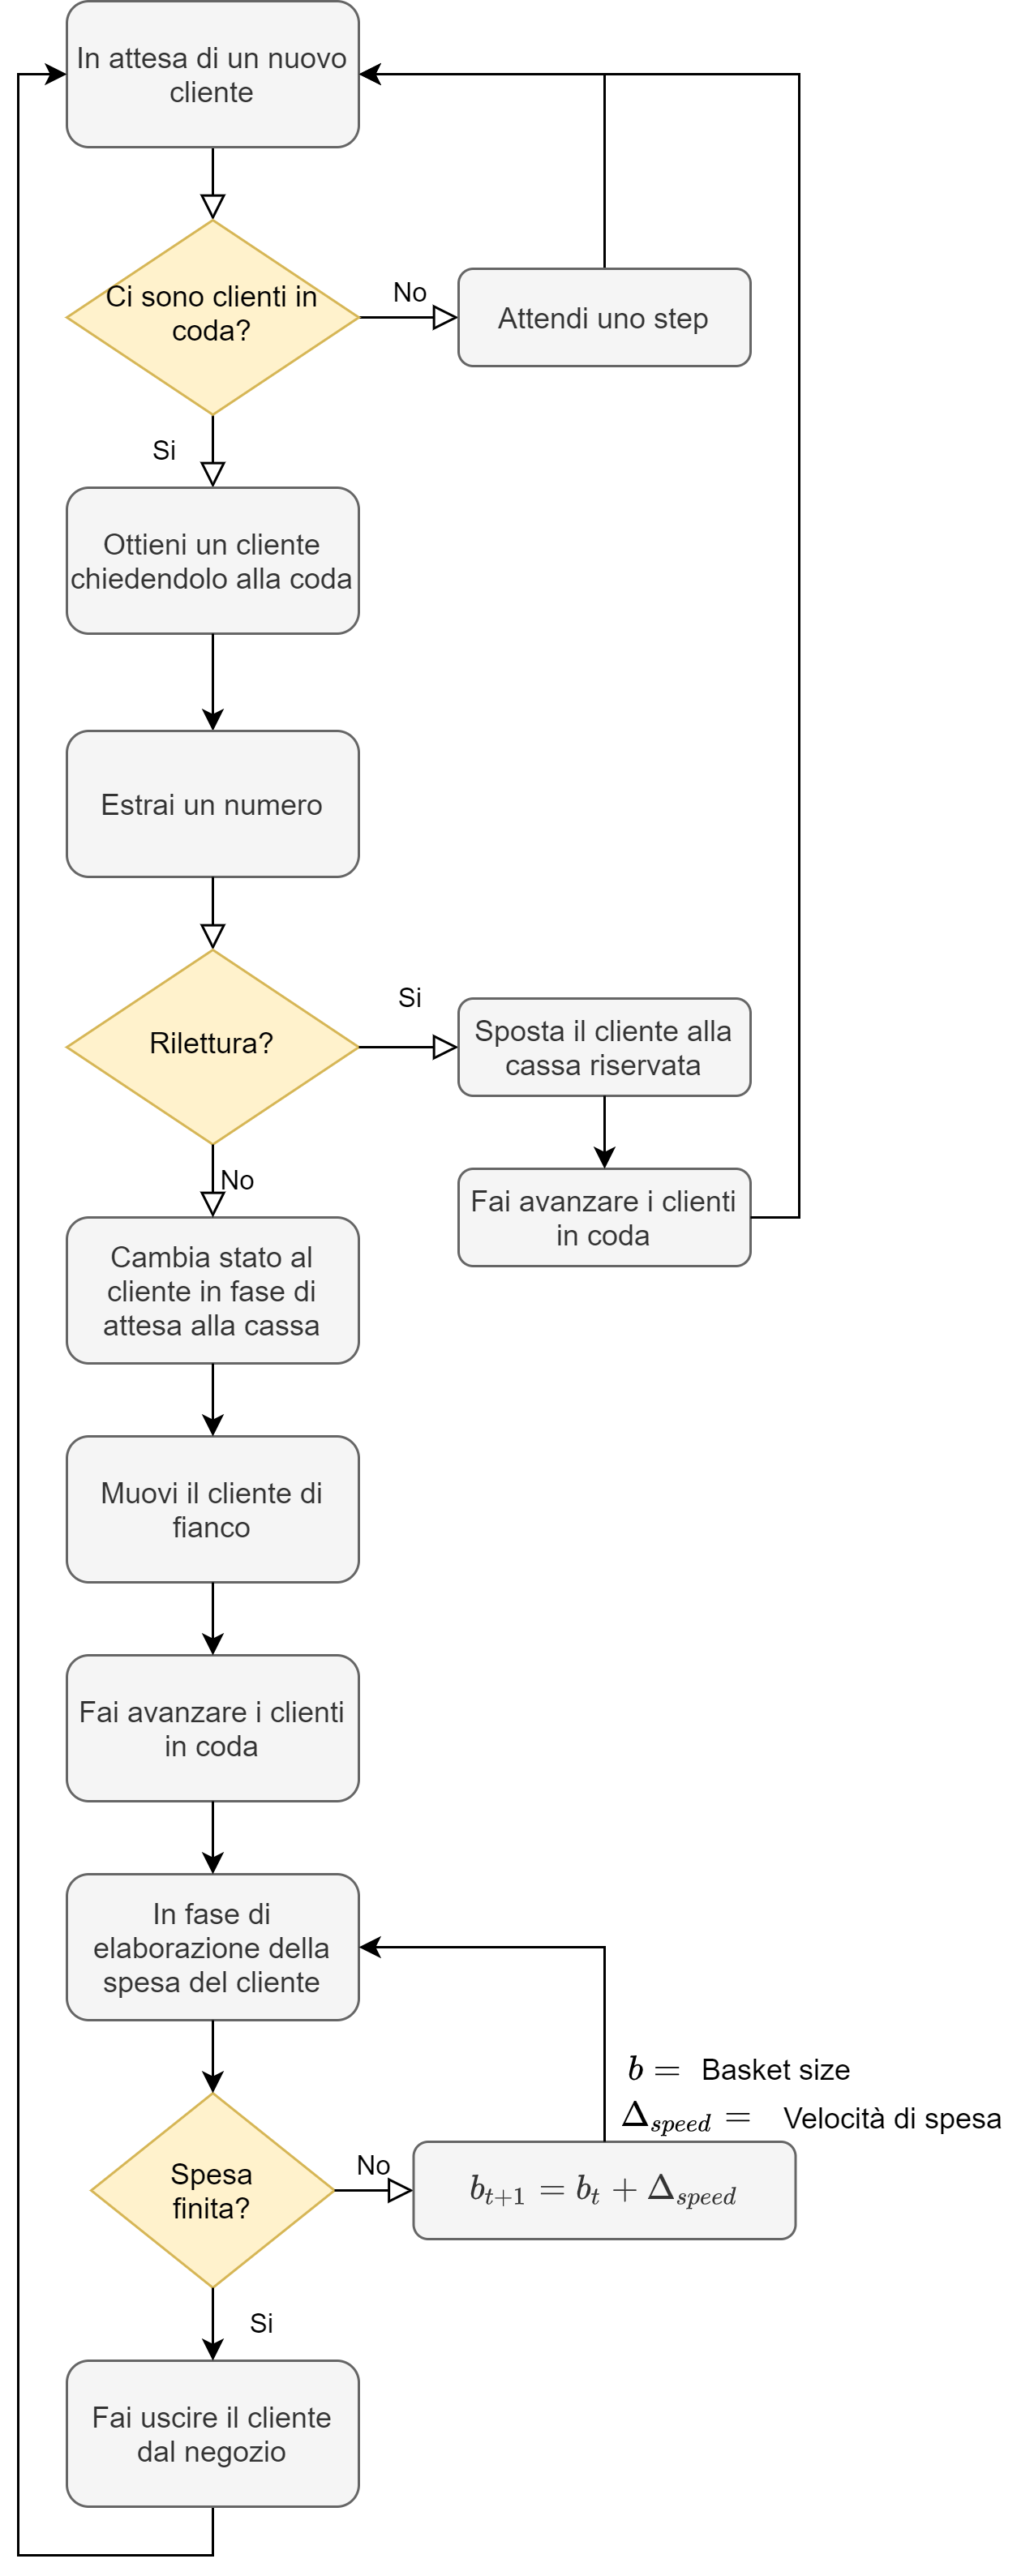
\includegraphics[width=8cm]{"images/workflow_cashdesk_self_scan.png"}
	\caption{Workflow dell'agente di tipo cassa self-scan.}
	\label{fig:workflow_cashdesk_self_scan}
\end{figure}

\paragraph{Cassa riservata}

Nella \textbf{fase di attesa di un nuovo cliente} la cassa riservata è pronta a servire i clienti in coda, però prima controlla che ci siano in coda clienti a cui è stata assegnata una rilettura parziale della spesa, dandogli la precedenza in quanto la rilettura parziale è più veloce di quella totale. \\
Scelto quindi il cliente, questa cassa passa per le stesse fasi della cassa standard.

Il workflow della cassa riservata viene riassunto nell'immagine \ref{fig:workflow_cashdesk_reserved}.

\begin{figure}[H]
	\centering
	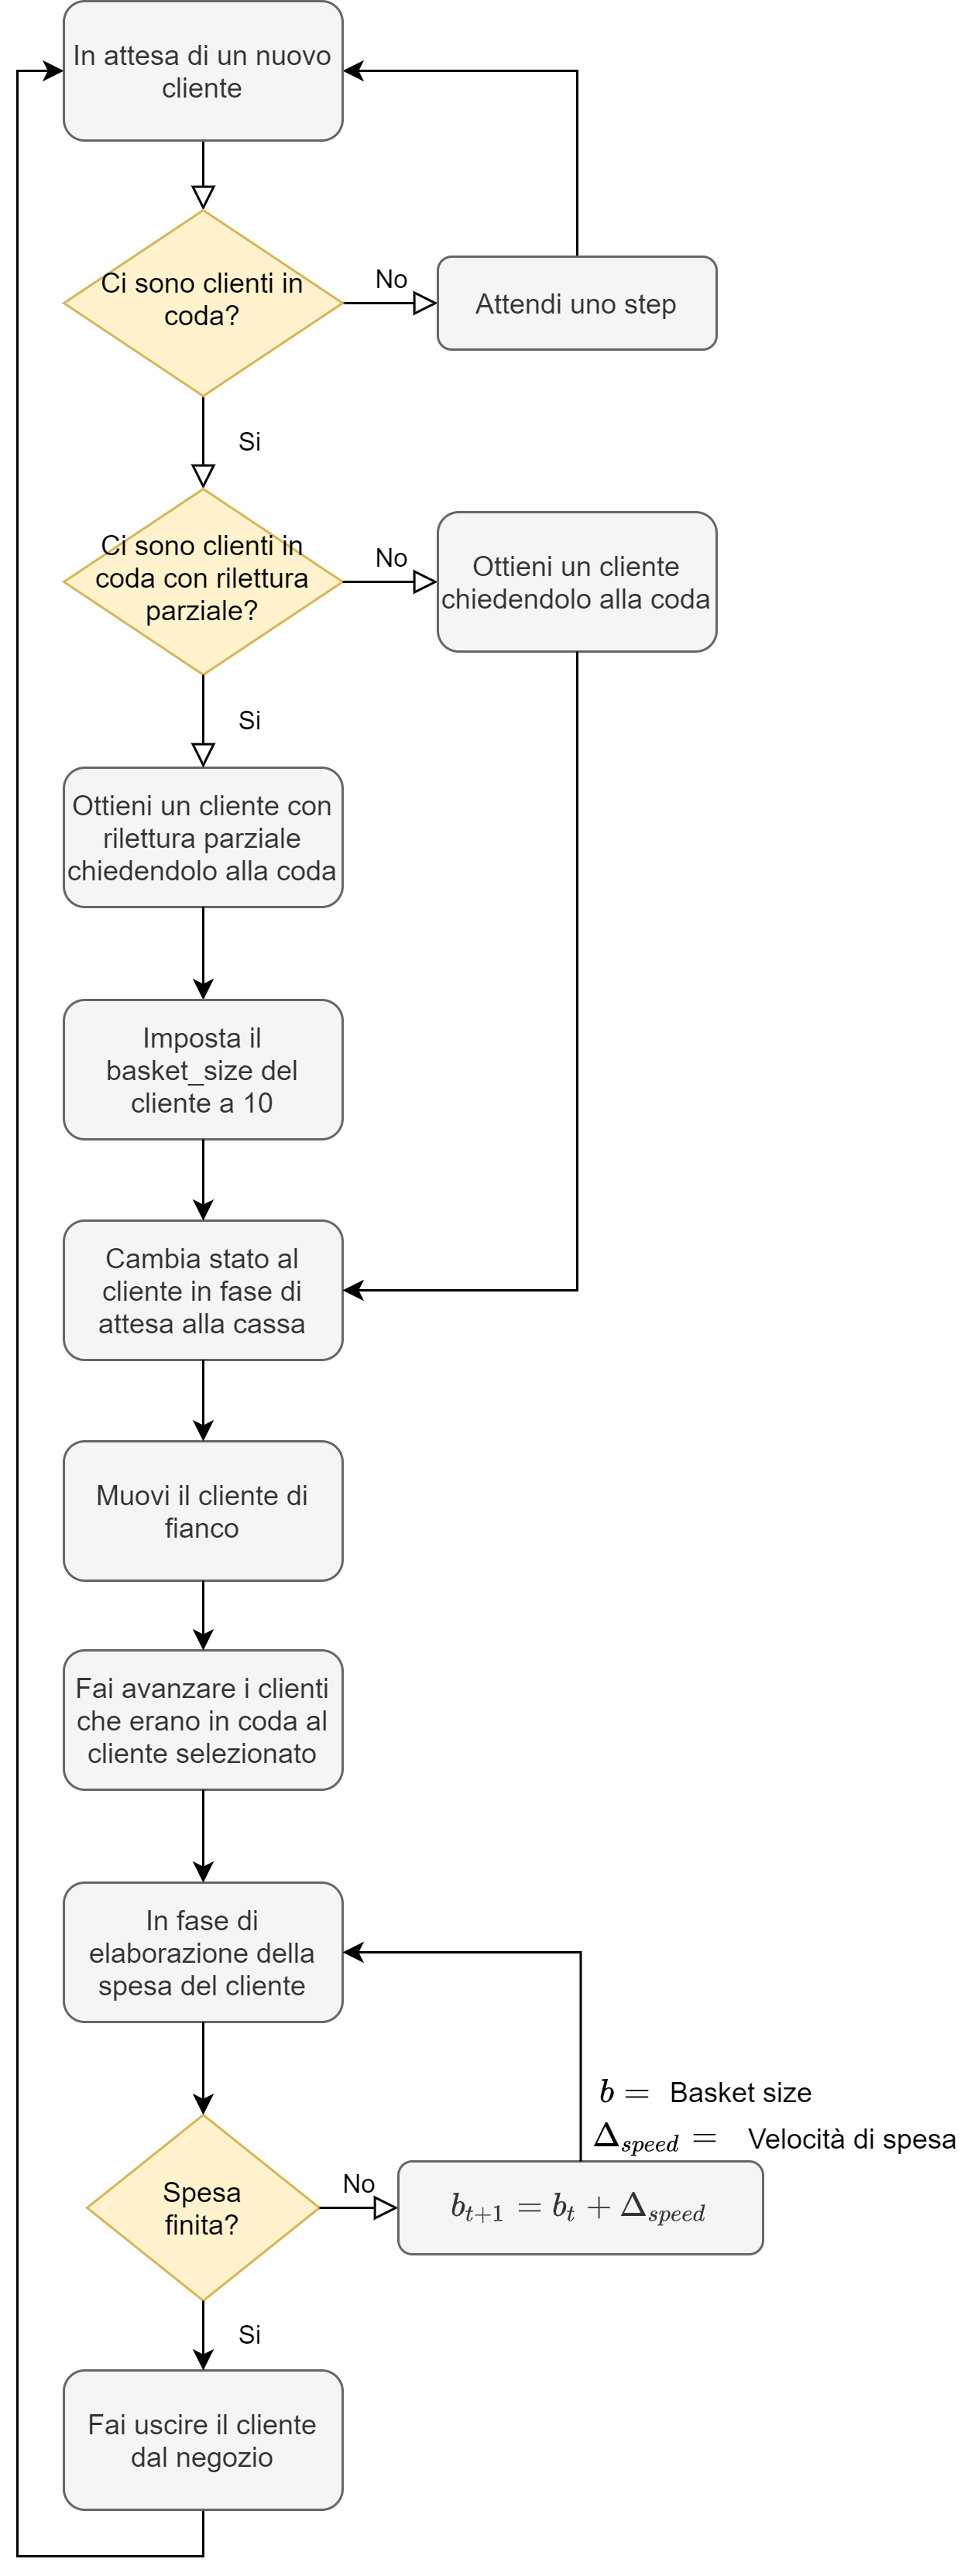
\includegraphics[width=8cm]{"images/workflow_cashdesk_reserved.png"}
	\caption{Workflow dell'agente di tipo cassa riservata.}
	\label{fig:workflow_cashdesk_reserved}
\end{figure}


\section{Ambiente}
\label{model:environment}

L'ambiente in cui gli agenti vivono è il supermercato, implementato dalla classe \textbf{Supermarket} che si occupa di inizializzare la griglia che verrà poi mostrata in fase di simulazione sull'interfaccia, inizializzare le casse, i clienti e mediare le interazioni con gli agenti.

Per inizializzare la griglia, l'ambiente viene diviso in zone: zona d'entrata, zona di shopping, zona casse normali, zona casse self-service, zona casse self-scan. Questa divisione permette una gestione più semplice dello spazio e dei movimenti degli agenti. Ogni zona ha come parametri la dimensione o il numero di casse che deve contenere, questi parametri vengono inizializzati a priori e gestiti dall'entry point del programma, il file \textbf{main}, come si vedrà nella prossima sezione.

Ogni zona è responsabile della propria costruzione, ovvero del proprio collocamento nella griglia dell'interfaccia in base alle proprie dimensioni ed eventualmente del posizionamento delle casse che contiene. Inoltre ogni zona è responsabile dei movimenti dei clienti: se un cliente vuole muoversi da una zona all'altra oppure mettersi in coda nelle casse di una zona, è la zona di destinazione che fornisce il metodo per posizionarsi correttamente in essa.


\begin{figure}[H]
	\centering
	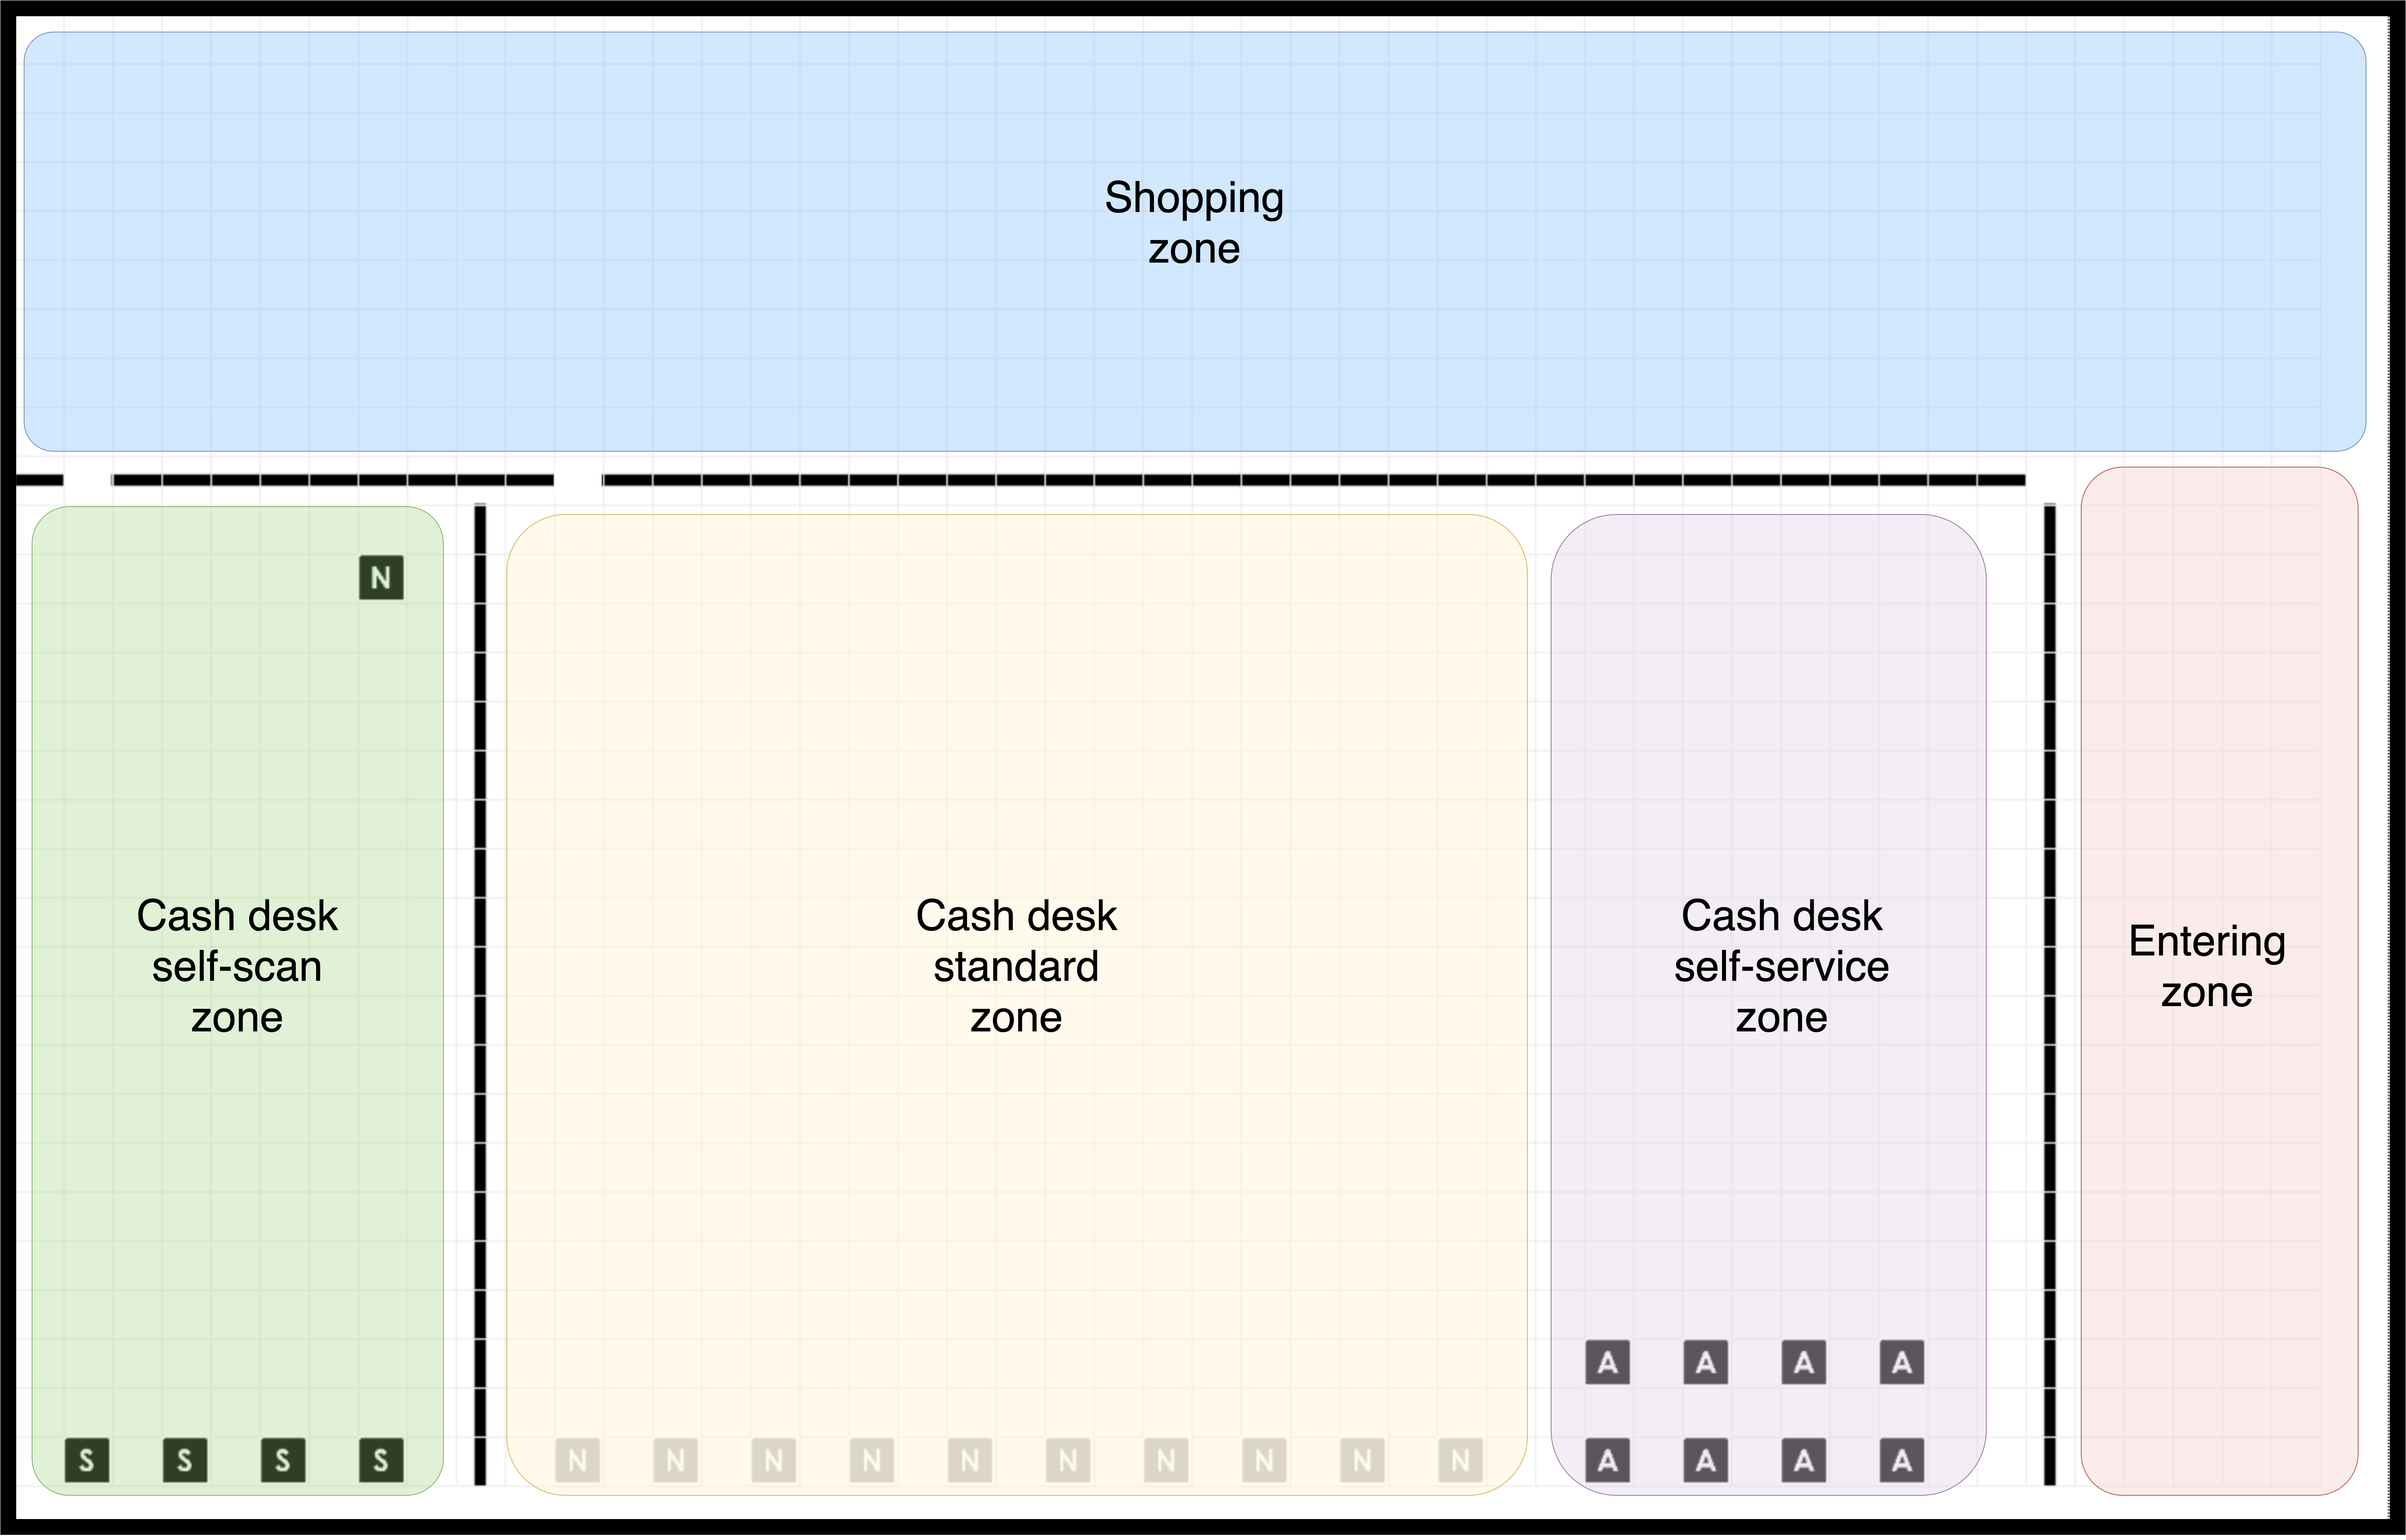
\includegraphics[width=14cm]{"images/supermarket-start-zones.png"}
	\caption{Stuttura del supermercato diviso in zone.}
	\label{fig:supermarket_zones}
\end{figure}


\todo{Parlare di quanto dura uno step e quanto dura una simulazione} Ad ogni step della simulazione, il modello crea dei clienti secondo la distribuzione data (si veda la sezione \ref{model:parameters}) e li posiziona nella \textbf{Entering Zone} del supermercato in coordinate random, dunque si occupa della attivazione e disattivazione delle casse standard in base al numero di clienti presenti nel negozio in quello step, secondo dei parametri che si vedranno nella prossima sezione. Quindi il modello chiama gli scheduler degli agenti, clienti e casse, e fa eseguire i loro step.

\subsection{Interazione tra agenti}

I due tipi di agenti che compongono il modello interagiscono tra loro nella fase di attesa in coda da parte del cliente e quindi pagamento; l'interazione è necessaria perchè i clienti non sono in grado di autogestire le code e pagare, e questo fatto giustifica la presenza degli agenti Cassa, pur semplici che siano (insieme al fatto che le casse si attivano o disattivano in base al numero di clienti nel negozio, come si vedrà più avanti).

L'interazione tra clienti e casse è di tipo \textbf{collaborativo semplice}, in quanto gli obiettivi di entrambi sono compatibili (effettuare il pagamento e far uscire i clienti dal negozio), le risorse sufficienti e le abilità insufficienti (i clienti non sanno fare da soli il pagamento e le casse non possono fare la spesa ai clienti). Le casse e i clienti collaborano e comunicano per raggiungere l'obiettivo.

Gli agenti sono a conoscenza di dove si trovano nell'ambiente, ma non vedono in modo diretto gli altri agenti e la distanza che li separa; se un agente di tipo Cliente prende una decisione su quale coda seguire, ha bisogno di chiedere al supermercato dove si trova questa coda. Come descritto sopra, il supermercato è diviso in zone, ogni zona è responsabile di comunicare agli agenti la propria posizione e le casse che contiene, quindi fornisce i metodi per muoversi in essa. Il mezzo attraverso cui gli agenti comunicano è dunque l'ambiente stesso.

\subsection{Caratteristiche dell'ambiente}

L'ambiente supermercato è per gli agenti totalmente \textbf{accessibile}, infatti i clienti sanno dove si trovano tutte le casse e le casse conoscono ad ogni istante il numero di clienti presenti nel negozio. \\
L'ambiente è \textbf{deterministico}, se gli agenti compiono un'azione (ad esempio se un cliente si muove verso una coda), si conosce a priori l'effetto dell'azione; l'evoluzione dell'ambiente è non deterministica, in quanto sono stati introdotti elementi aleatori nelle decisioni degli agenti. \\
Un'altra caratteristica dell'ambiente è l'\textbf{episodicità}, infatti le esperienze degli agenti, sia casse che clienti, sono divise in fasi il cui esito dipende soltanto dal presente e non dalla serie di azioni svolte in precedenza. \\
Il supermercato è un ambiente \textbf{statico} perchè non ha altri processi che operano oltre le casse e i clienti, che ci vivono dentro ma non lo modificano; non esistono interferenze nelle azioni degli agenti. \\
Infine l'ambiente è \textbf{discreto}, esistono un numero finito di azioni da effettuare, ma anche dal punto di vista fisico esso è rappresentato da una griglia di celle finite.

\section{Considerazioni sul modello}

Il modello é stato sviluppato in modo da essere flessibile per
permettere con semplicità future espansioni e cambiamenti. Gli aspetti
più dinamici del modello, ovvero il comportamento degli agenti, le
varie modalità di scelta di una coda e la capacità di un agente
Cliente di effettuare \textit{jockeying} sono stati realizzati lasciando
all'utilizzatore piena possibilità di modifica, ampliamento o di non
utilizzo. A livello di architettura del software questo si traduce
nell'implementazione dei pattern:

\begin{itemize}
\item \textbf{Strategy}: usato per definire diverse modalità di scelta
  della coda e diversi comportamenti di \textit{jockeying}. Nuovi comportamenti possono essere aggiunti rispettando un'interfaccia standard. Permette se necessario cambiamenti di comportamento a run time.
\item \textbf{State}: usato per definire tramite una macchina a stati
  finiti i comportamenti degli agenti Cliente e Cassa. Nuovi stati
  possono essere aggiunti con facilità e collegati ad altri stati
  tramite transizioni. La divisione in stati rende semplice ragionare
  sul comportamento di un agente.
\end{itemize}

\section{Parametri del modello}
\label{model:parameters}

Per rendere il modello più generale possibile e in modo da adattarlo a diverse configurazioni con lo scopo di simulare scenari what-if, vengono introdotti diversi parametri per l'inizializzazione e il comportamento della simulazione.
\todo{Controllare questo paragrafo pls}

\subsection{Configurazione delle casse e struttura del supermercato}
Tra i parametri più importanti e con maggiore impatto per il modello troviamo sicuramente la \textbf{configurazione del supermercato}. Un primo fattore che caratterizza la struttura del supermercato  è la dimensione delle diverse zone: \textit{shopping zone}, \textit{cash-desk zone} e \textit{entering zone}.

Ancora più influente e determinante per il comportamento del modello è il numero e tipo di casse che compongono il supermercato. Infatti una volta scelta la struttura e le dimensioni delle diverse zone, è necessario indicare nella \textit{cash-desk zone} il numero di casse per ogni tipo, quindi specificare la quantità di:
\begin{itemize}
	\item Casse self-scan (+ 1 riservata obbligatoria)
	\item Casse standard
	\item Casse self-service
\end{itemize}

Inoltre è necessario specificare un'ulteriore parametro che definisce se le casse di tipo standard hanno delle code parallele o una coda condivisa tra tutte; questo non avviene per le casse self-scan e self-service, in quanto nel primo caso c'è sempre una coda condivisa unica, e nel secondo c'è sempre una coda ogni 8 casse.

\subsection{Parametri di jockeying}
Il comportamento di jockeying è influenzato da alcuni parametri, questi sono:
\begin{itemize}
	\item \textbf{Numero di code adiacenti considerate}: la coda in cui il customer è presente in quel momento svolge il ruolo di coda pivot, questo parametro indica il numero di code adiacenti alla coda pivot che vengono prese in considerazione per valutare l'eventualità di fare jockeying.
	\item \textbf{Threshold di jockeying}: questo parametro ha lo scopo di modellare il fatto che un cliente efettua jockeying solo nel caso in cui per lui risulta essere conveniente non meno di un certo livello; questo threshold indica quale deve essere il minimo guadagno per effettuare jockeying. Questo approccio basato su una soglia di minimo guadagno è stato presentato nel lavoro di Koenigsberg \cite{koenigsberg1966jockeying}.
	\item \textbf{Probabilità di jockeying}: nel lavoro di Tomasz Antczak e altri \cite{article1}, viene spiegato come il fenomeno di jockeying sia piuttosto raro. Il modello proposto tiene conto di questo aspetto introducendo una variabile aleatoria bernoulliana che ha lo scopo di consentire o negare il jockeying, nel caso in cui il jockeying risulti essere conveniente basandosi sul threshold. Con questo approccio si vuole rendere meno frequente il jockeying.
\end{itemize}

\subsection{Basket size}
Ogni cliente all'interno del supermercato vuole comprare un diverso numero di prodotti. Questa quantità viene assegnata a priori per tutti i clienti e supponiamo non cambi durante la fase di spesa; a questo scopo è necessario assegnare il basket size a ogni cliente secondo una certa distribuzione. Nel lavoro di Antczak e altri \cite{article1} vengono messi a disposzione dei dati relativi al numero di prodotti acquistati da parte dei clienti in tre supermercati diversi nell'arco temporale di 13 giorni. Questi dati sono stati analizzati con lo scopo di introdurre la distribuzione che genera il basket size di ogni cliente.

Come prima cosa è stata presa in considerazione la frequenza delle dimensioni del basket size per ogni negozio al variare del tempo. Disegnando in un grafico queste informazioni si ottiene l'immagine \ref{fig:3d_basket_size}.

\begin{figure}[H]
	\centering
	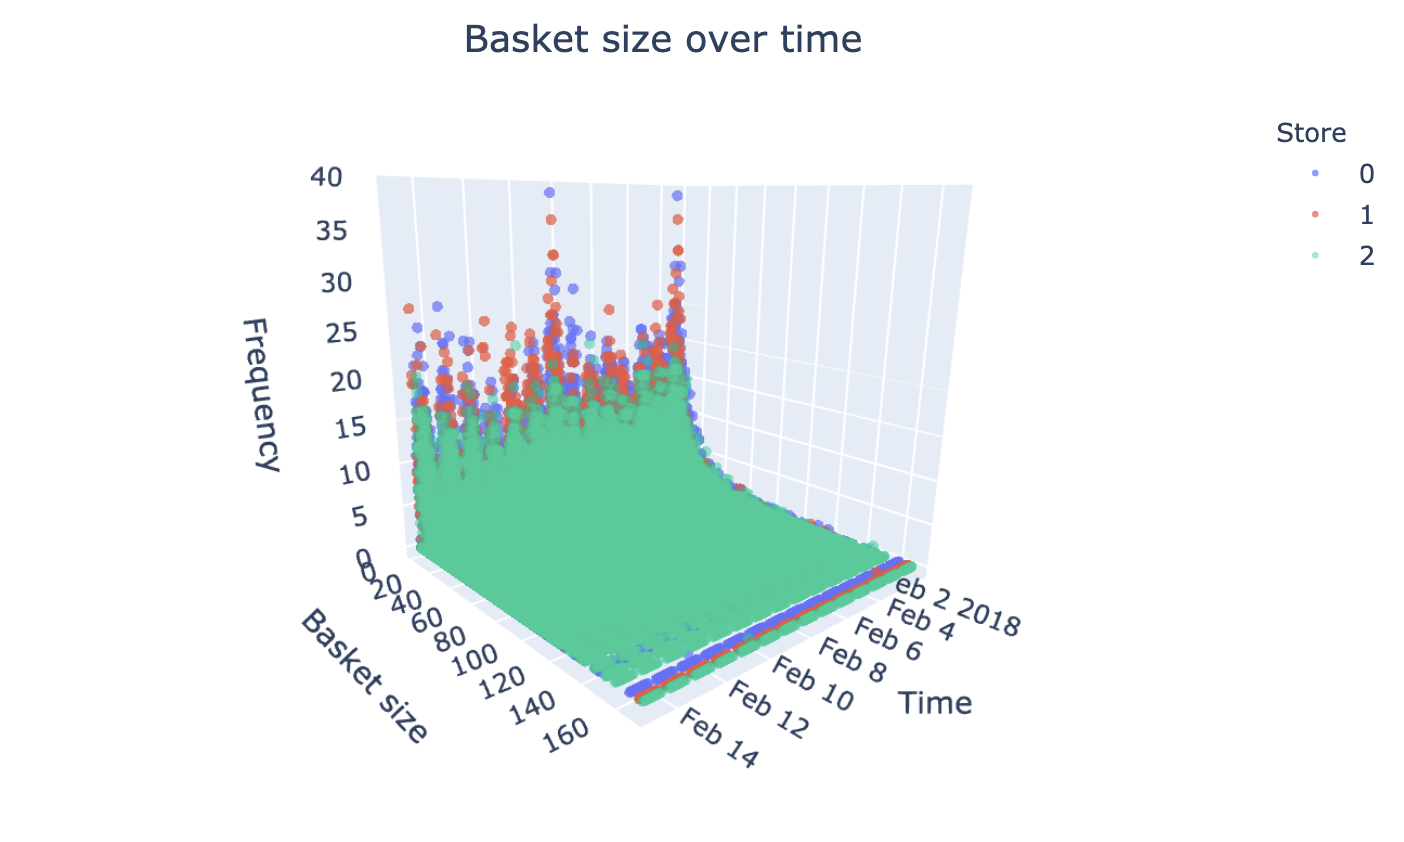
\includegraphics[width=14cm]{"images/3d_basket_size.png"}
	\caption{Frequenza della dimensione del basket size nei supermercati al variare del tempo.}
	\label{fig:3d_basket_size}
\end{figure}

Da questa immagine emerge chiaramente come la maggior parte delle persone compra pochi articoli e solo pochi clienti fanno una grossa spesa. Inoltre il comportamento tra i 3 supermercati è analogo a meno del numero di clienti totali del supermercato. Per quanto riguarda i diversi giorni considerati nell'arco di tempo messo a disposizione, non sembra che questi influiscano sulla dimensione del basket size, pertanto assumiamo per semplicità che non esista una correlazione tra i giorni della settimana e la dimensione del basket size.

Con questa assunzione si procede aggregando i dati sulla dimensione del tempo e calcolando la media, inoltre questi dati vengono normalizzati per renderli \textit{scale-free} e quindi indipendenti dal numero di clienti per ogni supermercato. Dopo queste operazioni si ottiene il grafico \ref{fig:store_basket_size}.

\begin{figure}[H]
	\centering
	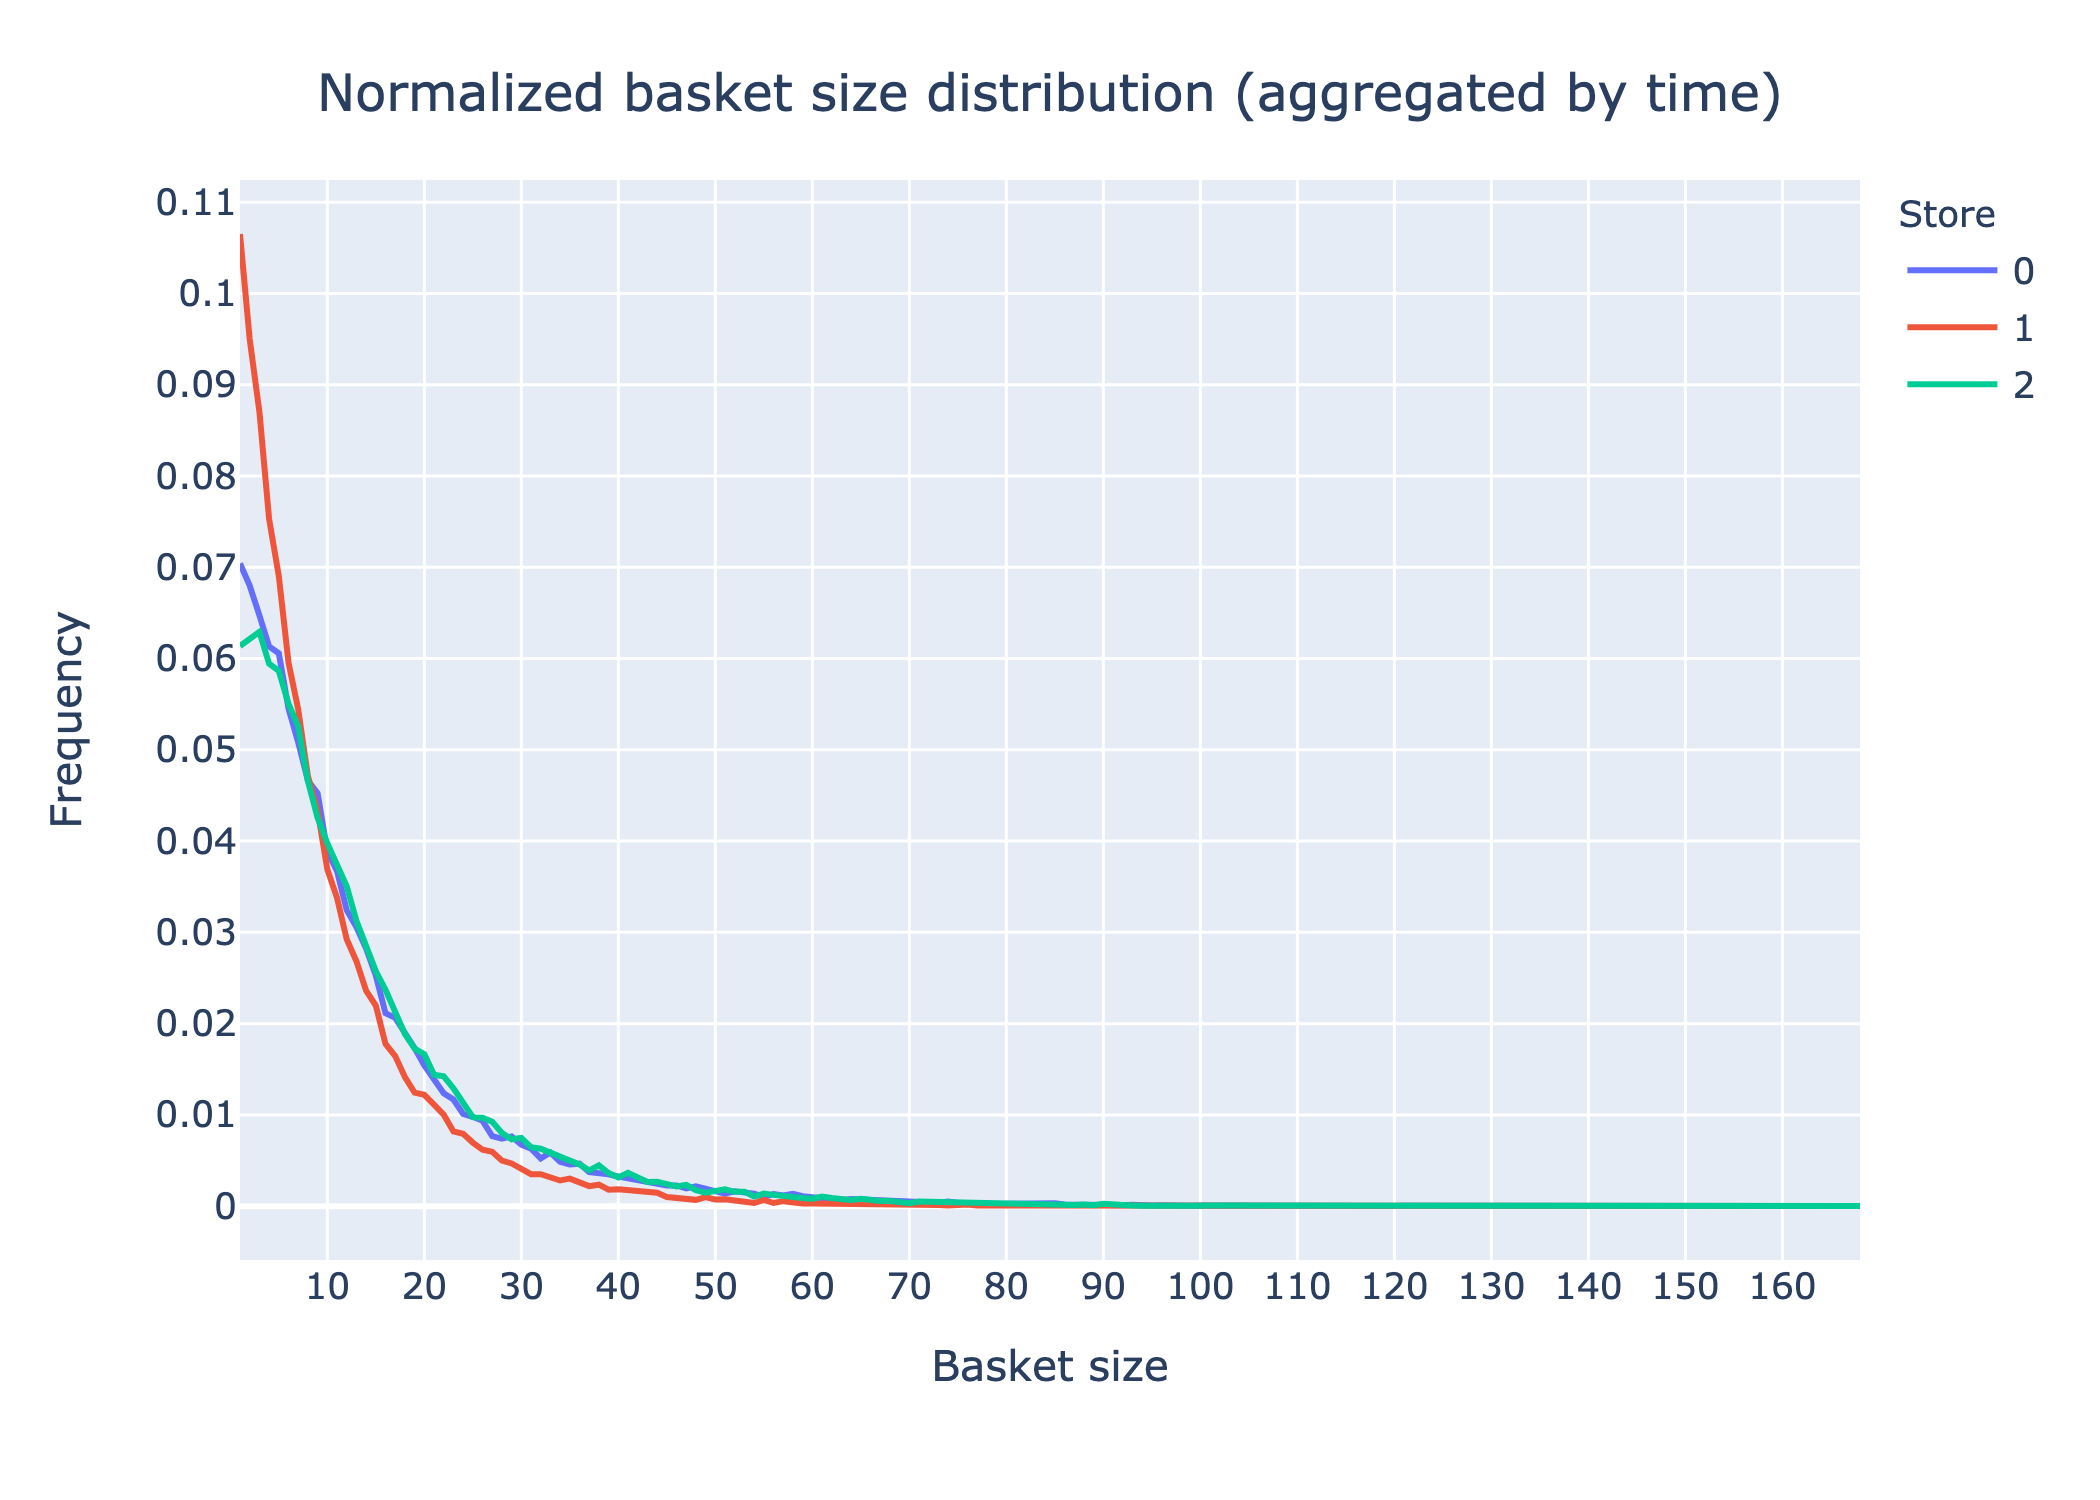
\includegraphics[width=14cm]{"images/basket_size_dist.png"}
	\caption{Frequenza della dimensione del basket size nei supermercati aggregato sul tempo.}
	\label{fig:store_basket_size}
\end{figure}

Notiamo come le distribuzioni nei 3 supermercati siano in generale simili, per questa ragione vengono mediate le 3 distribuzioni ottenendo questa la distribuzione finale \ref{fig:avg_basket_size}.

\begin{figure}[H]
	\centering
	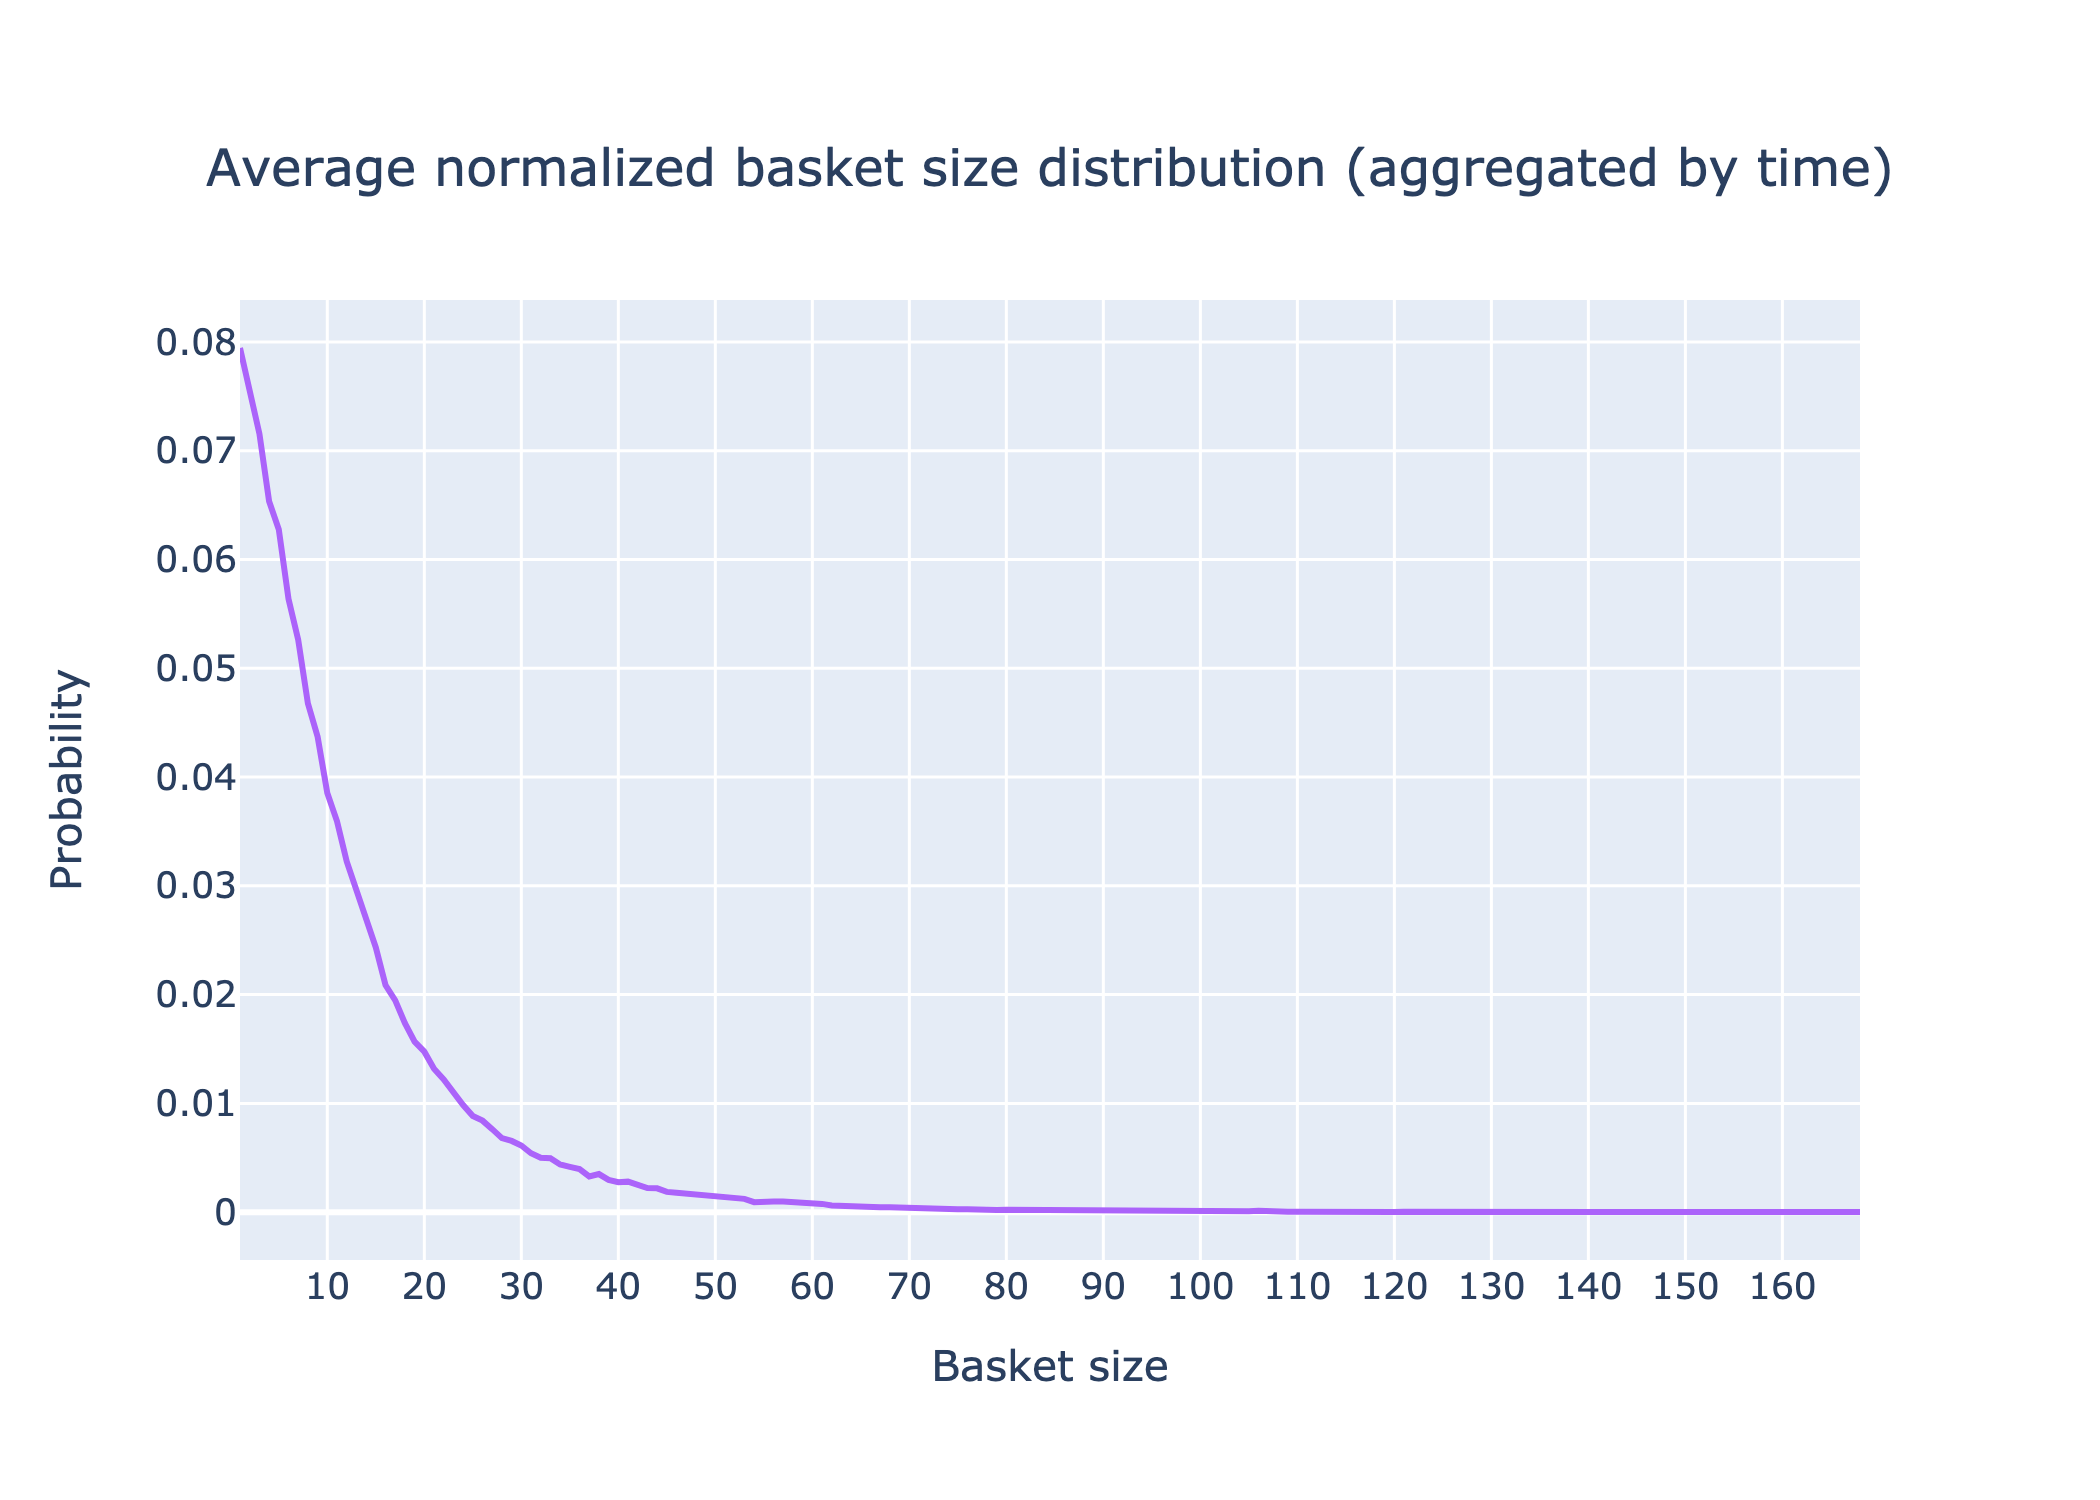
\includegraphics[width=14cm]{"images/basket_size_dist_avg.png"}
	\caption{Media delle distribuzioni di frequenza del basket size aggregato sul tempo.}
	\label{fig:avg_basket_size}
\end{figure}

Da questa ultima immagine emerge chiaramente come la probabilità del basket size segua un andamento esponenziale, pertanto a partire dai dati originali si vuole ricavare il parametro $\lambda$ che governa la distribuzione esponenziale sottostante. A questo scopo si trasformano i dati calcolando il logaritmo naturale delle ascisse e tracciando la retta di regressione lineare. Il risultato ottenuto viene mostrato nell'immagine \ref{fig:regression_log}.

\begin{figure}[H]
	\centering
	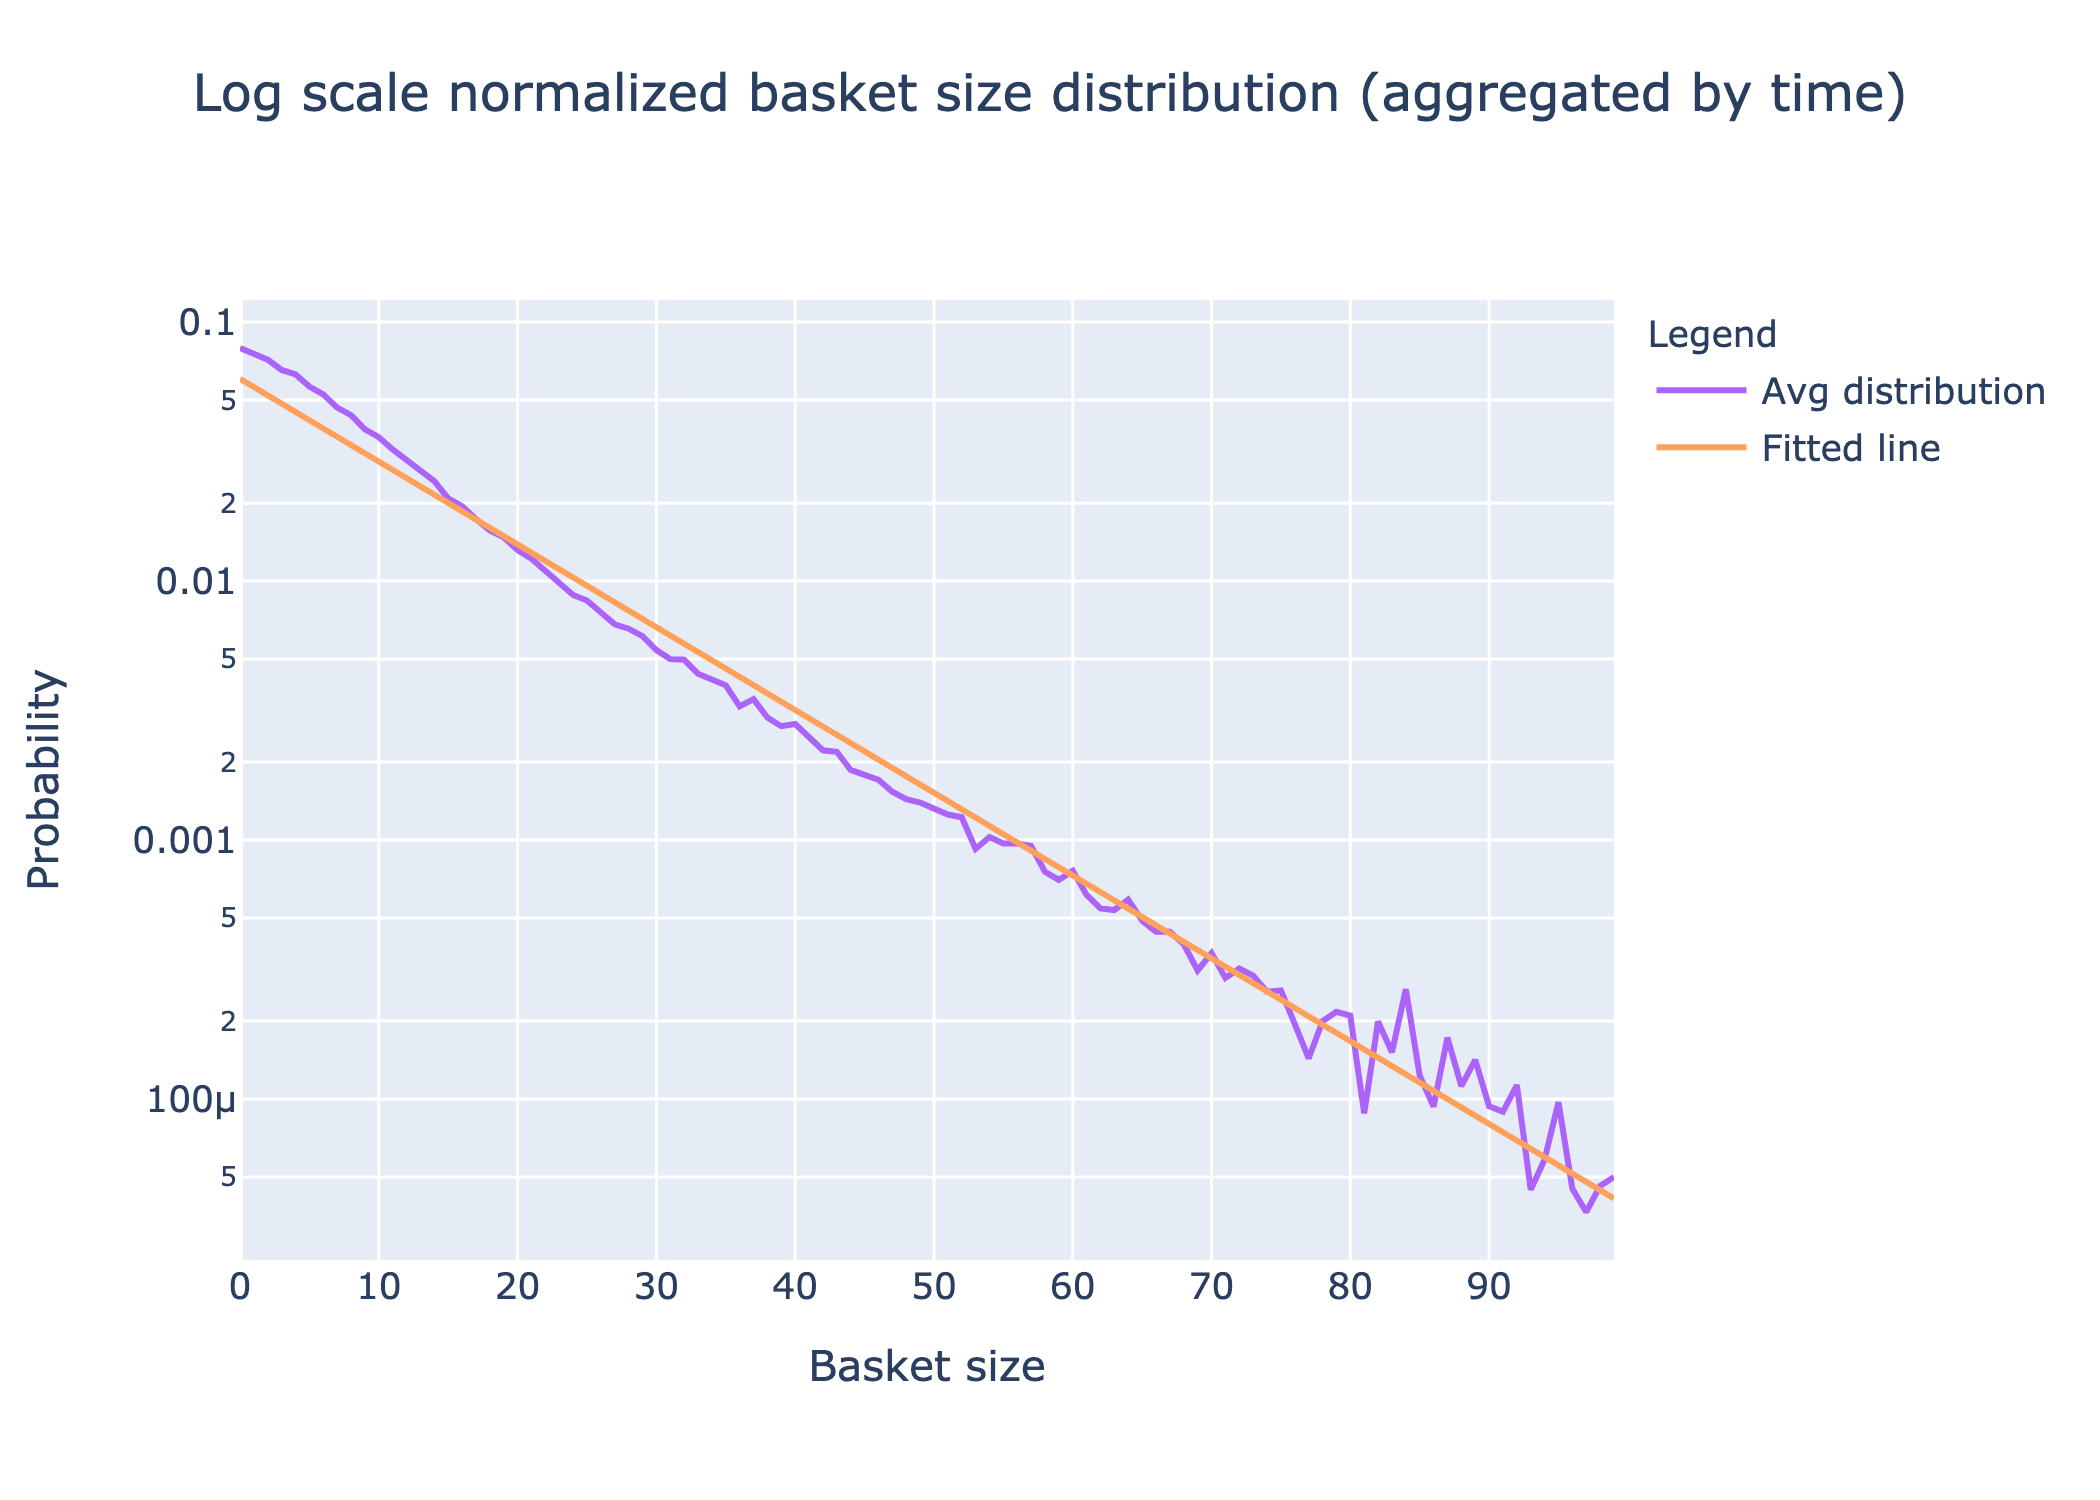
\includegraphics[width=14cm]{"images/basket_size_log.png"}
	\caption{Retta di regressione dopo la trasformazione logaritmica dei dati.}
	\label{fig:regression_log}
\end{figure}

La retta di regressione in output ha i seguenti parametri:
\begin{itemize}
	\item $m = -0.0736184654254411$
	\item $q = -2.806857867915933$
\end{itemize}
A partire da questi parametri è facile calcolare il parametro $\lambda$ della distribuzione esponenziale di partenza, infatti:

\begin{proof}[\unskip\nopunct]
	Sia $X$ la variabile aleatoria che rappresenta la dimensione del basket size, e assumendo che $X \sim Exp(\lambda)$, dalla funzione di densità di probabilità si ha che:
	$$f(x;\lambda) = \lambda e^{\lambda x}, \quad se \; x > 0$$

	Per mezzo di una log-trasformazione si ottiene:

	\begin{equation}
			\label{eq:regressione}
		\begin{aligned}
			&\ln(\lambda e^{\lambda x}) &&\text{(dalla funzione di densità di probabilità)}\\
			&= \ln(\lambda) + \ln(e^{-\lambda x}) \\
			&= \ln(\lambda) - \lambda x \ln(e) \\
			&= \ln(\lambda) - \lambda x \\
		\end{aligned}
	\end{equation}

	La retta di regressione ottenuta a parire dai dati dopo la log-trasformazione è della forma:
	\begin{align*}
		&y = mx + q\\
		&m = -0.0736184654254411;\, q = -2.806857867915933
	\end{align*}

	Da cui (sfruttando l'equazione \ref{eq:regressione}):
		\begin{align*}
			&m = -\lambda \implies \lambda = -m = 0.0736184654254411\\
			&q = \ln(\lambda)\\
		\end{align*}

	Pertanto si ricava dai dati che la distribuzione esponenziale teorica sottostante $Exp(\lambda)$ ha $\lambda = 0.0736184654254411$.
\end{proof}

Nella figura \ref{fig:dist_basket_size} viene mostrata la distribuzione reale dei dati e la distribuzione esponenziale, la quale verrà poi effettivamente utilizzata per generare il basket size di ogni cliente:

\begin{figure}[H]
	\centering
 	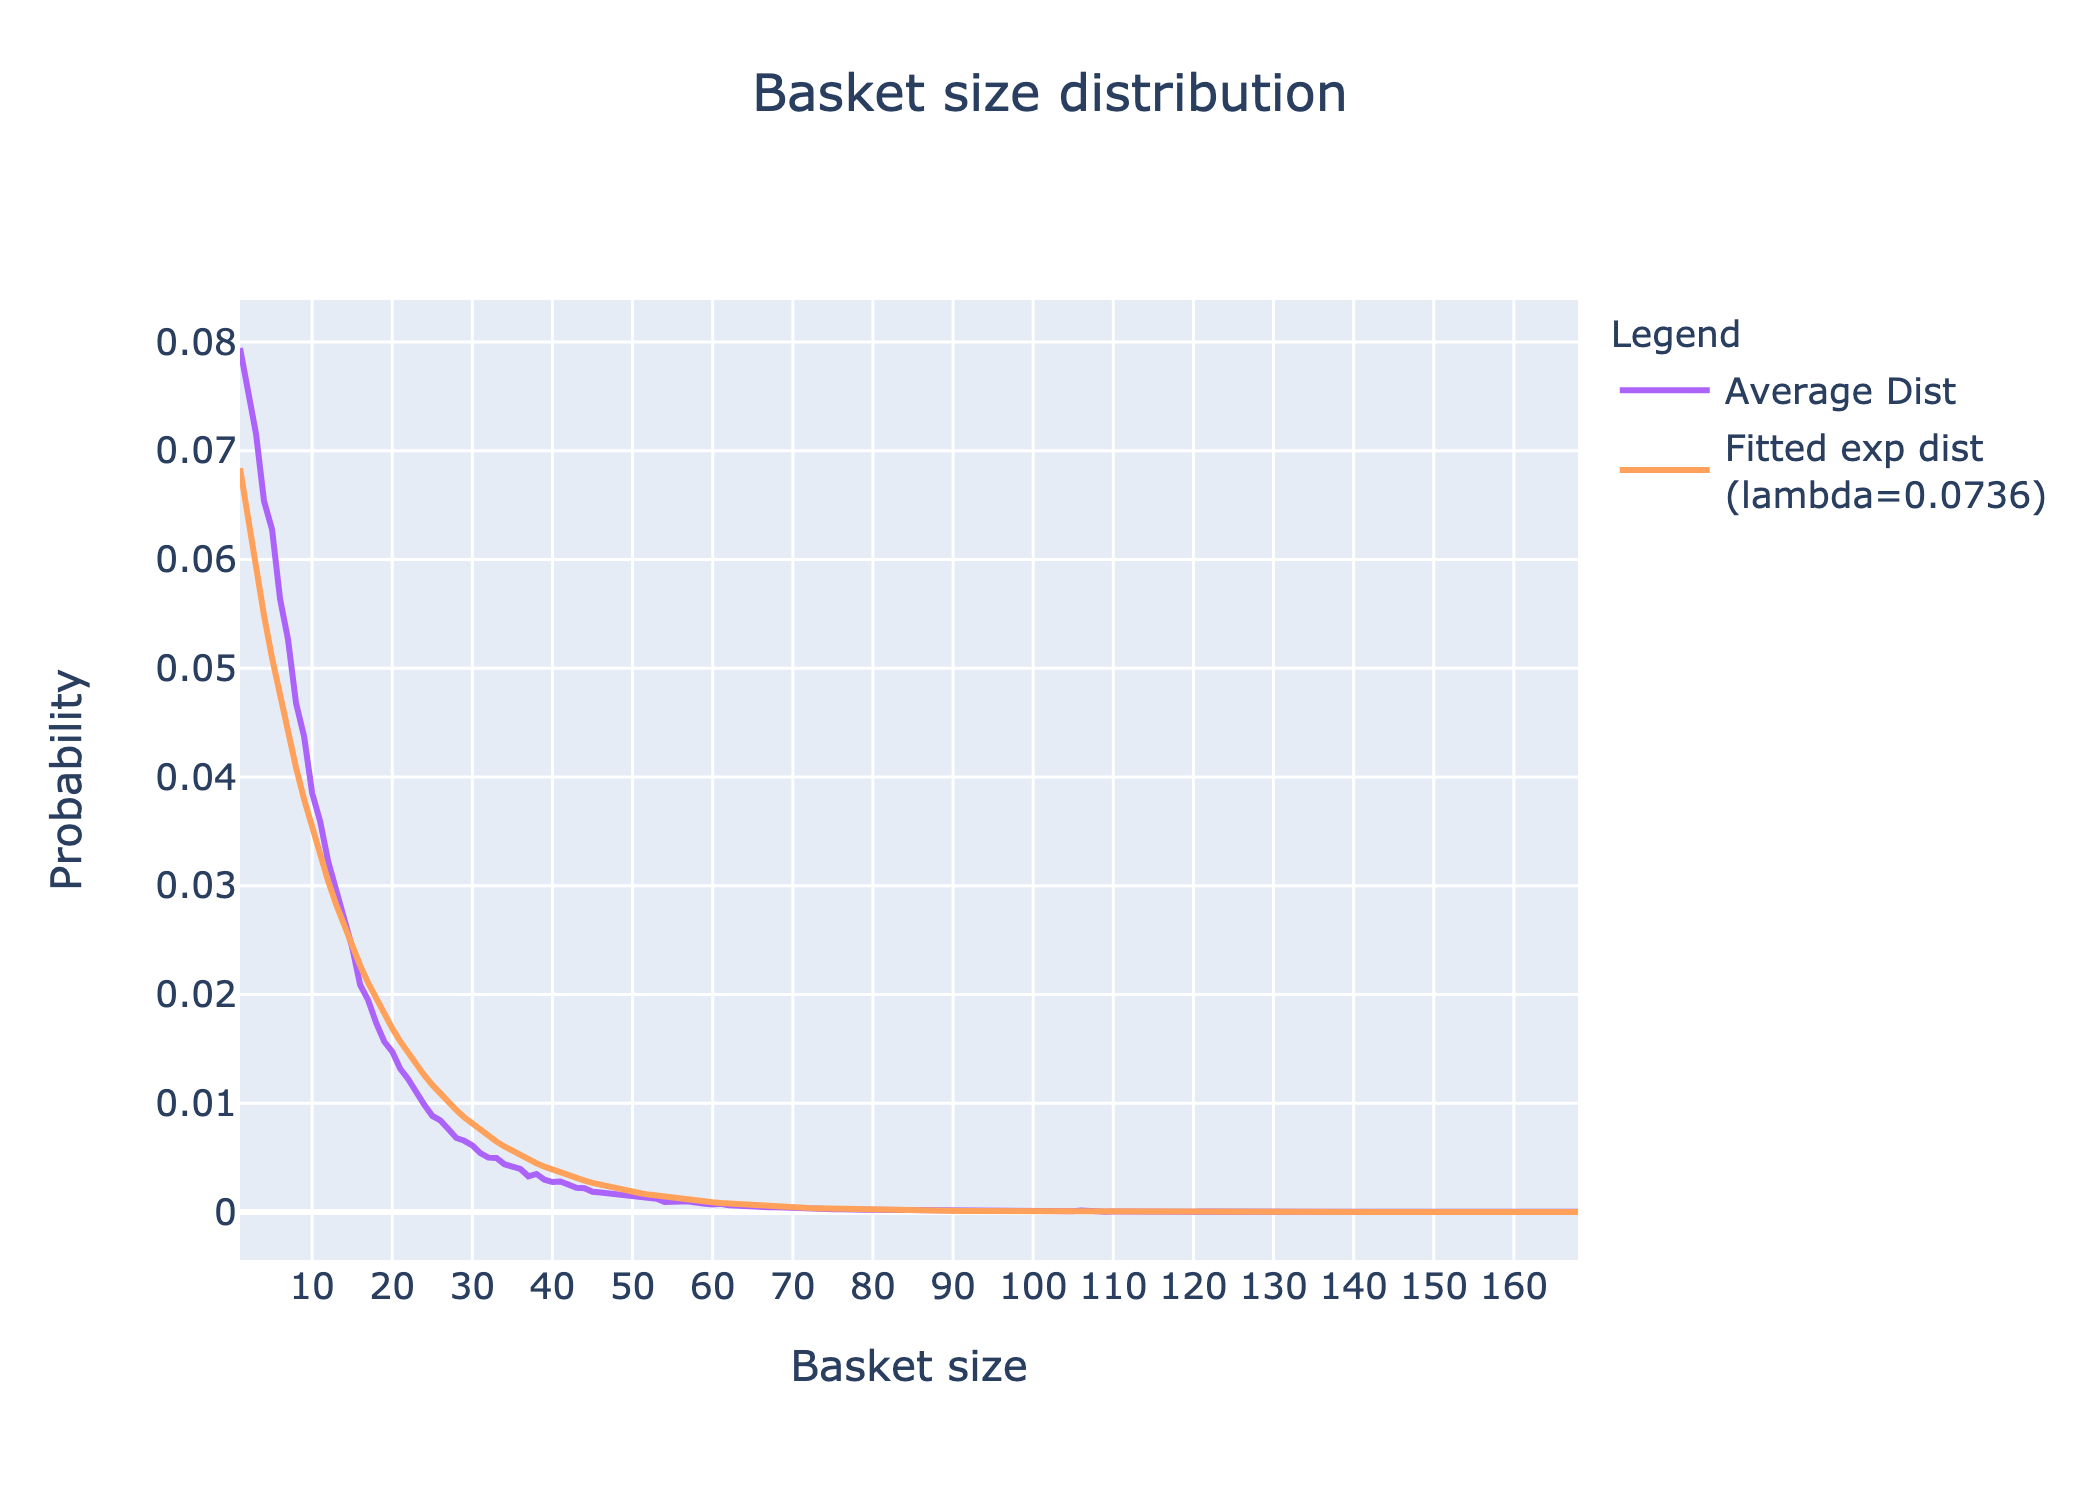
\includegraphics[width=14cm]{"images/basket_size_fitted.png"}
	\caption{Distribuzione basket size reale a confronto con distribuzione esponenziale teorica.}
	\label{fig:dist_basket_size}
\end{figure}

\subsection{Parametri di tempo}
\label{parameters:time}
Lo scorrere del tempo all'interno del modello viene simulato per mezzo di step. Per questo motivo è necessario scegliere uno step del modello a quanti secondi corrisponde. Per le simulazioni effettuate nel nostro lavoro è stato scelto che \textbf{uno step corrisponde a 30 secondi}.

Come visto nel workflow dell'agente di tipo cliente, riassunto nell'immagine \ref{fig:workflow_customer}, una volta che egli entra nel supermercato è necessario simulare il processo di spesa del cliente, con questo si intende l'arco di tempo che l'agente impiega all'interno del supermercato per prendere i prodotti e inserirli nel carrello (che in questo lavoro non viene direttamente modellato ma simulato). Il tempo impiegato da parte del cliente per prendere tutti i prodotti desiderati, quantità che corrisponde al suo basket size, dipende dalla velocità di acquisto del cliente. Questa velocità è un ulteriore parametro del modello, che al momento è pari a \todo{Inserire a quanti prodotti corrisponde la velocità e quindi cosa si vuole simulare (es 2 prodotti al minuto)}

Dopo la fase di spesa iniziale il cliente sceglie una coda per venire successivamente servito in cassa. Una volta in cassa, se questa è di tipo cassa standard o cassa self-service, introdotte nella sezione \ref{sec:tipi_cassa}, allora è necessario processare tutto il basket size; quindi il cliente esce dal supermercato. \todo{Spiegare la velocità di processamento per le casse normali} Il tempo di elaborazione della spesa e governato dai parametri $a,b,\alpha ,\beta \in \mathbb{R}$  introdotti nell'articolo \cite{article1} e diversi per i due tipi di casse. Come questi parametri influiscono il tempo di processamento del cliente una volta in cassa è spiegato nella sezione \ref{sec:tipi_cassa}.

\subsection{Distibuzione dei clienti in entrata nel supermercato}
Nel lavoro di Antczak e altri \cite{article1}, oltre ai dati relativi al basket size di ogni cliente, vengono messi a disposizione i dati degli arrivi dei clienti per ogni supermercato analizzato. I dati raccolti fanno riferimento a 13 giorni: dal "1 febbraio 2018" al "14 febbraio 2018" e si considera il supermercato aperto per  14 ore (dalle 8:00 ale 22:00).

La distribuzione dei clienti in ingresso rappresenta l'attività all'interno del supermercato viene mostrata in figura \ref{fig:shop_activity}
 
 
\begin{figure}[H]
	\centering
	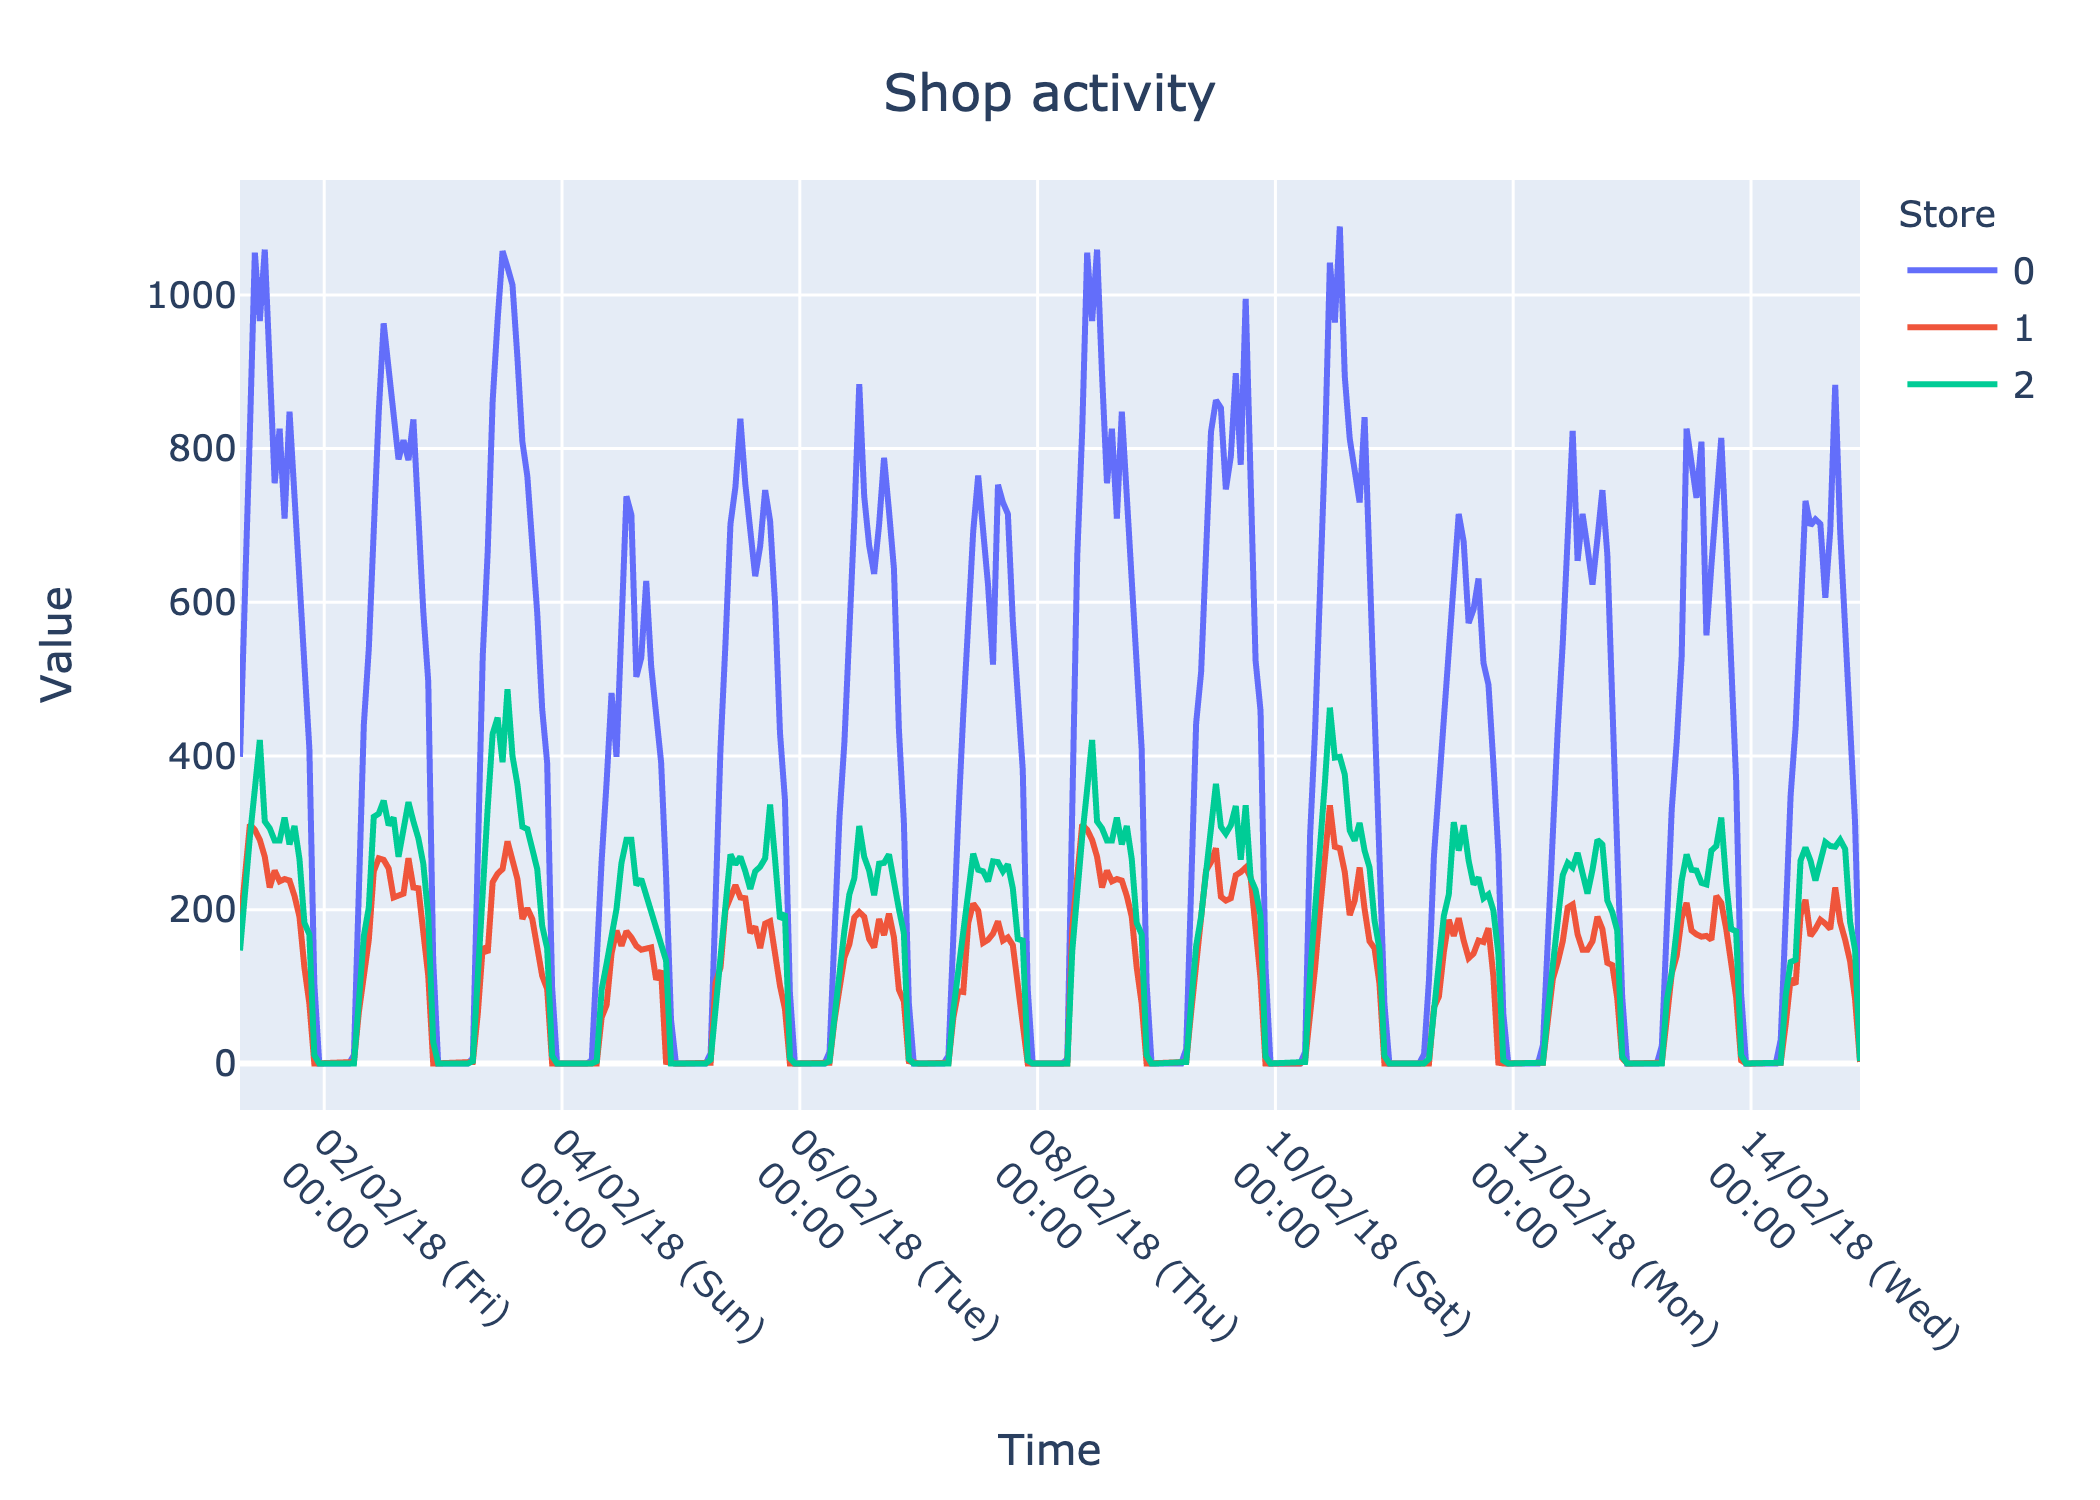
\includegraphics[width=14cm]{"images/shop_activity.png"}
	\caption{Distribuzione dei clienti in ingressi per ogni supermercato.}
	\label{fig:shop_activity}
\end{figure}

La distribuzione dei clienti in ingresso dipende dal numero di clienti totali nell'arco dell'intera giornata. Per rendere la distribuzione indipendete da questo fattore, vengono nomalizzate le distribuzioni per il numero totale di clienti. Il risultato viene mostrato in figura \ref{fig:shop_activity_normalized}

\begin{figure}[H]
	\centering
	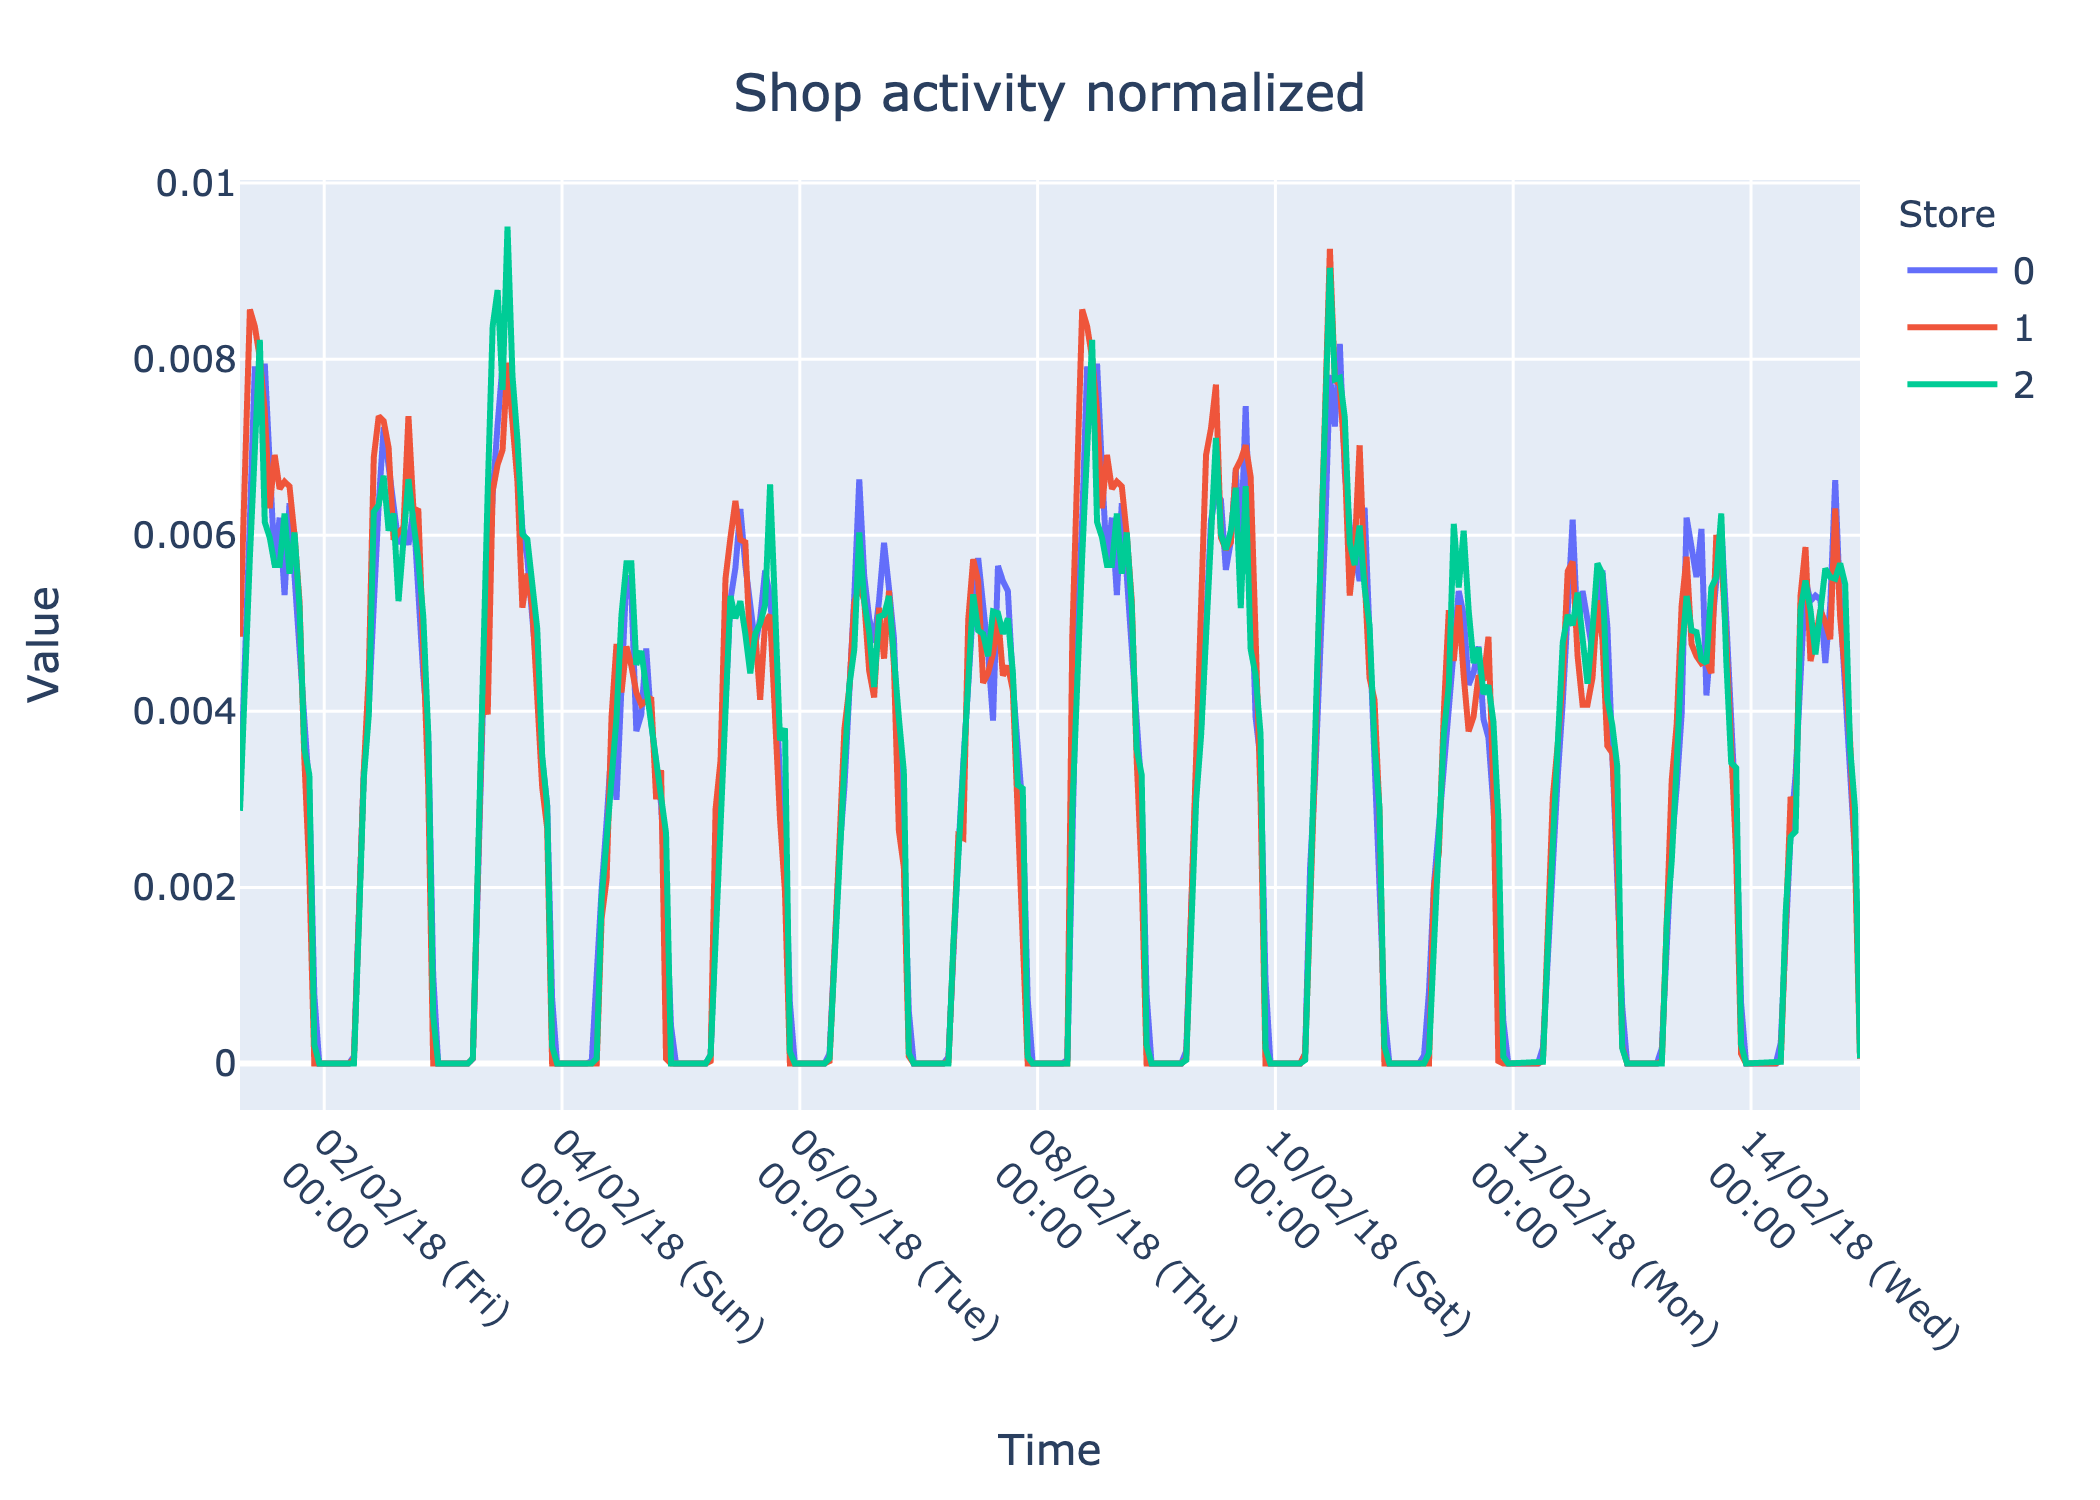
\includegraphics[width=14cm]{"images/shop_activity_normalized.png"}
	\caption{Distribuzione normalizzata dei clienti in ingressi per ogni supermercato.}
	\label{fig:shop_activity_normalized}
\end{figure}

Dalla figura  \ref{fig:shop_activity_normalized} si nota come le distribuzioni nei supermercati, normalizzando per i clienti totali in ingresso nell'arco della giornata, è molto simile e quindi assumiamo che possa valere per un supermercato in generale.

Si procede aggregando gli ingressi al variare delle diverse giorante e calcolando la media. Dopo questa operazione si ottengono le tre distribuzioni dei diversi supermercati, più una ottenuta dalla media di queste tre. Il risultato viene mostrato in figura \ref{fig:shop_activity_aggregated}, dove notiamo come la linea viola corrisponde alla media delle tre distribuzioni, questa distribuzione verrà usata come parametro per specificare gli ingressi durante le simulazioni al variare del tempo.


\begin{figure}[H]
	\centering
	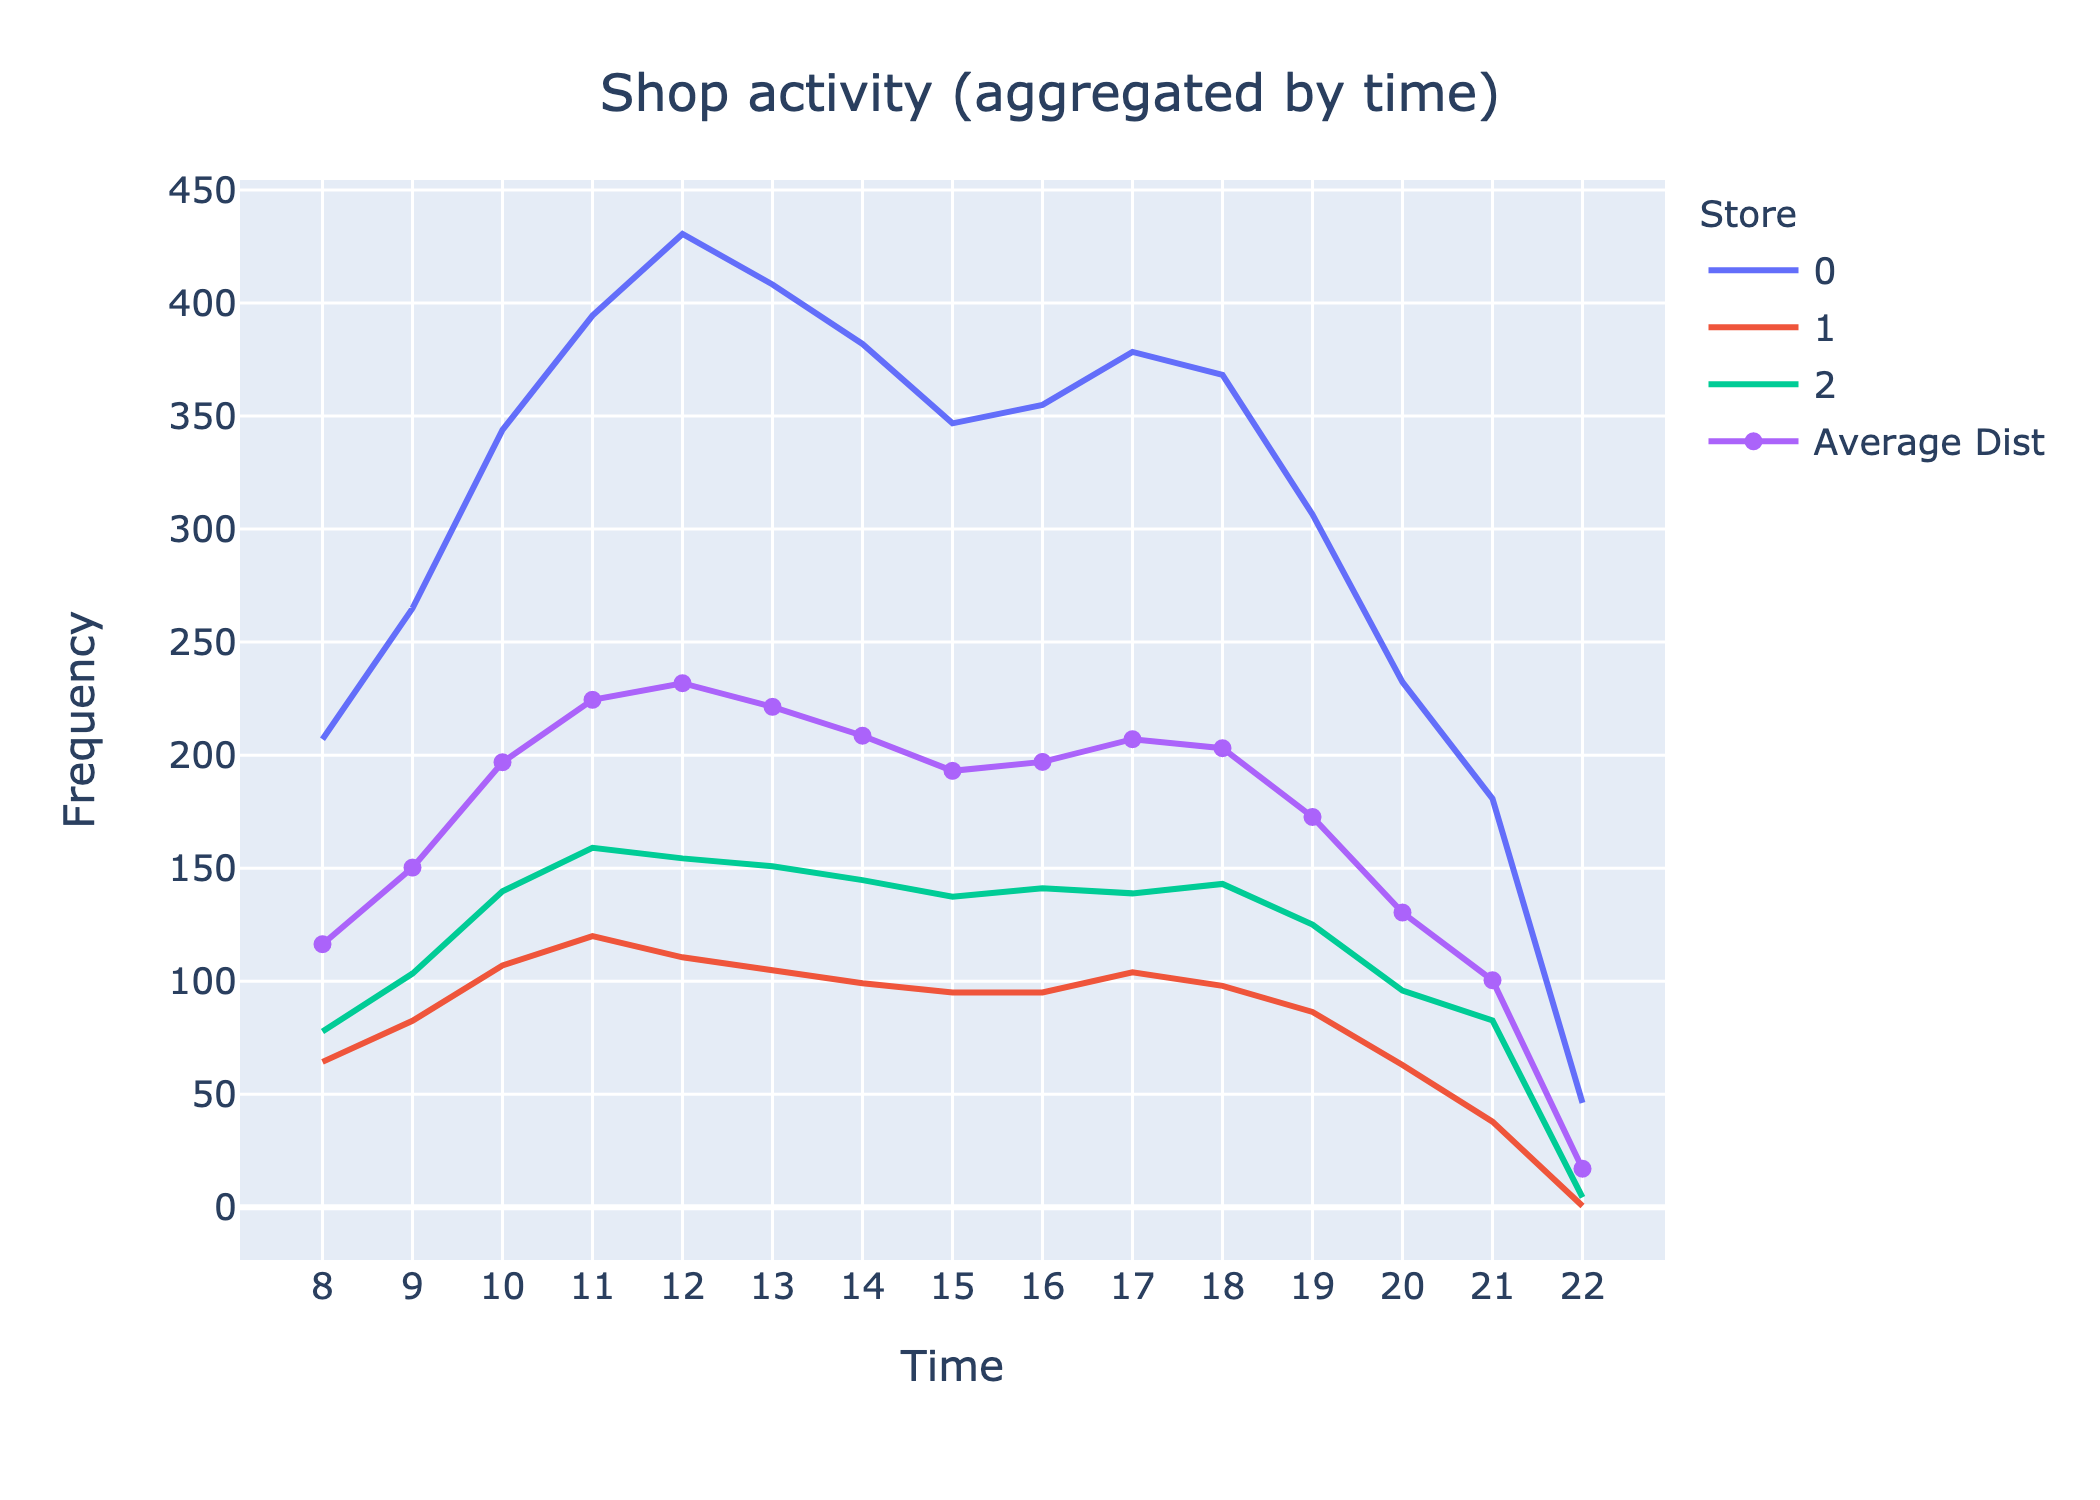
\includegraphics[width=14cm]{"images/shop_activity_aggregated.png"}
	\caption{Distribuzione dei clienti in ingressi aggregata per diversi giorni.}
	\label{fig:shop_activity_aggregated}
\end{figure}


Un ulteriore fattore da considerare è che nei dati a nostra dipsosizione gli ingressi dei clienti sono aggregati per ora, tuttavia durante la simulazioni è necessario fare entrare i clienti gradualmente ad ogni ora, ovvero gestire gli ingressi ad ogni step del modello. A questo scopo abbiamo considerato come distribuzione di riferimento quell ottenuta medianto le tre distribuzioni aggregate per i diversi giorni (linea viola nell'immagine \ref{fig:shop_activity_aggregated}). Dal momento che ad uno step del modello corrisponde a 30 secondi reali (spiegato qui \ref{parameters:time}), un'ora è composta da 120 steps. Con questa osservazione è possibile calcolare il valore atteso di clienti in entrata per ogni step al variare delle ore.

Il valore atteso di clienti in ingresso per ogni step al variare delle ore viene mostrato nella figura \ref{fig:per_step_distribution}.

\begin{figure}[H]
	\centering
	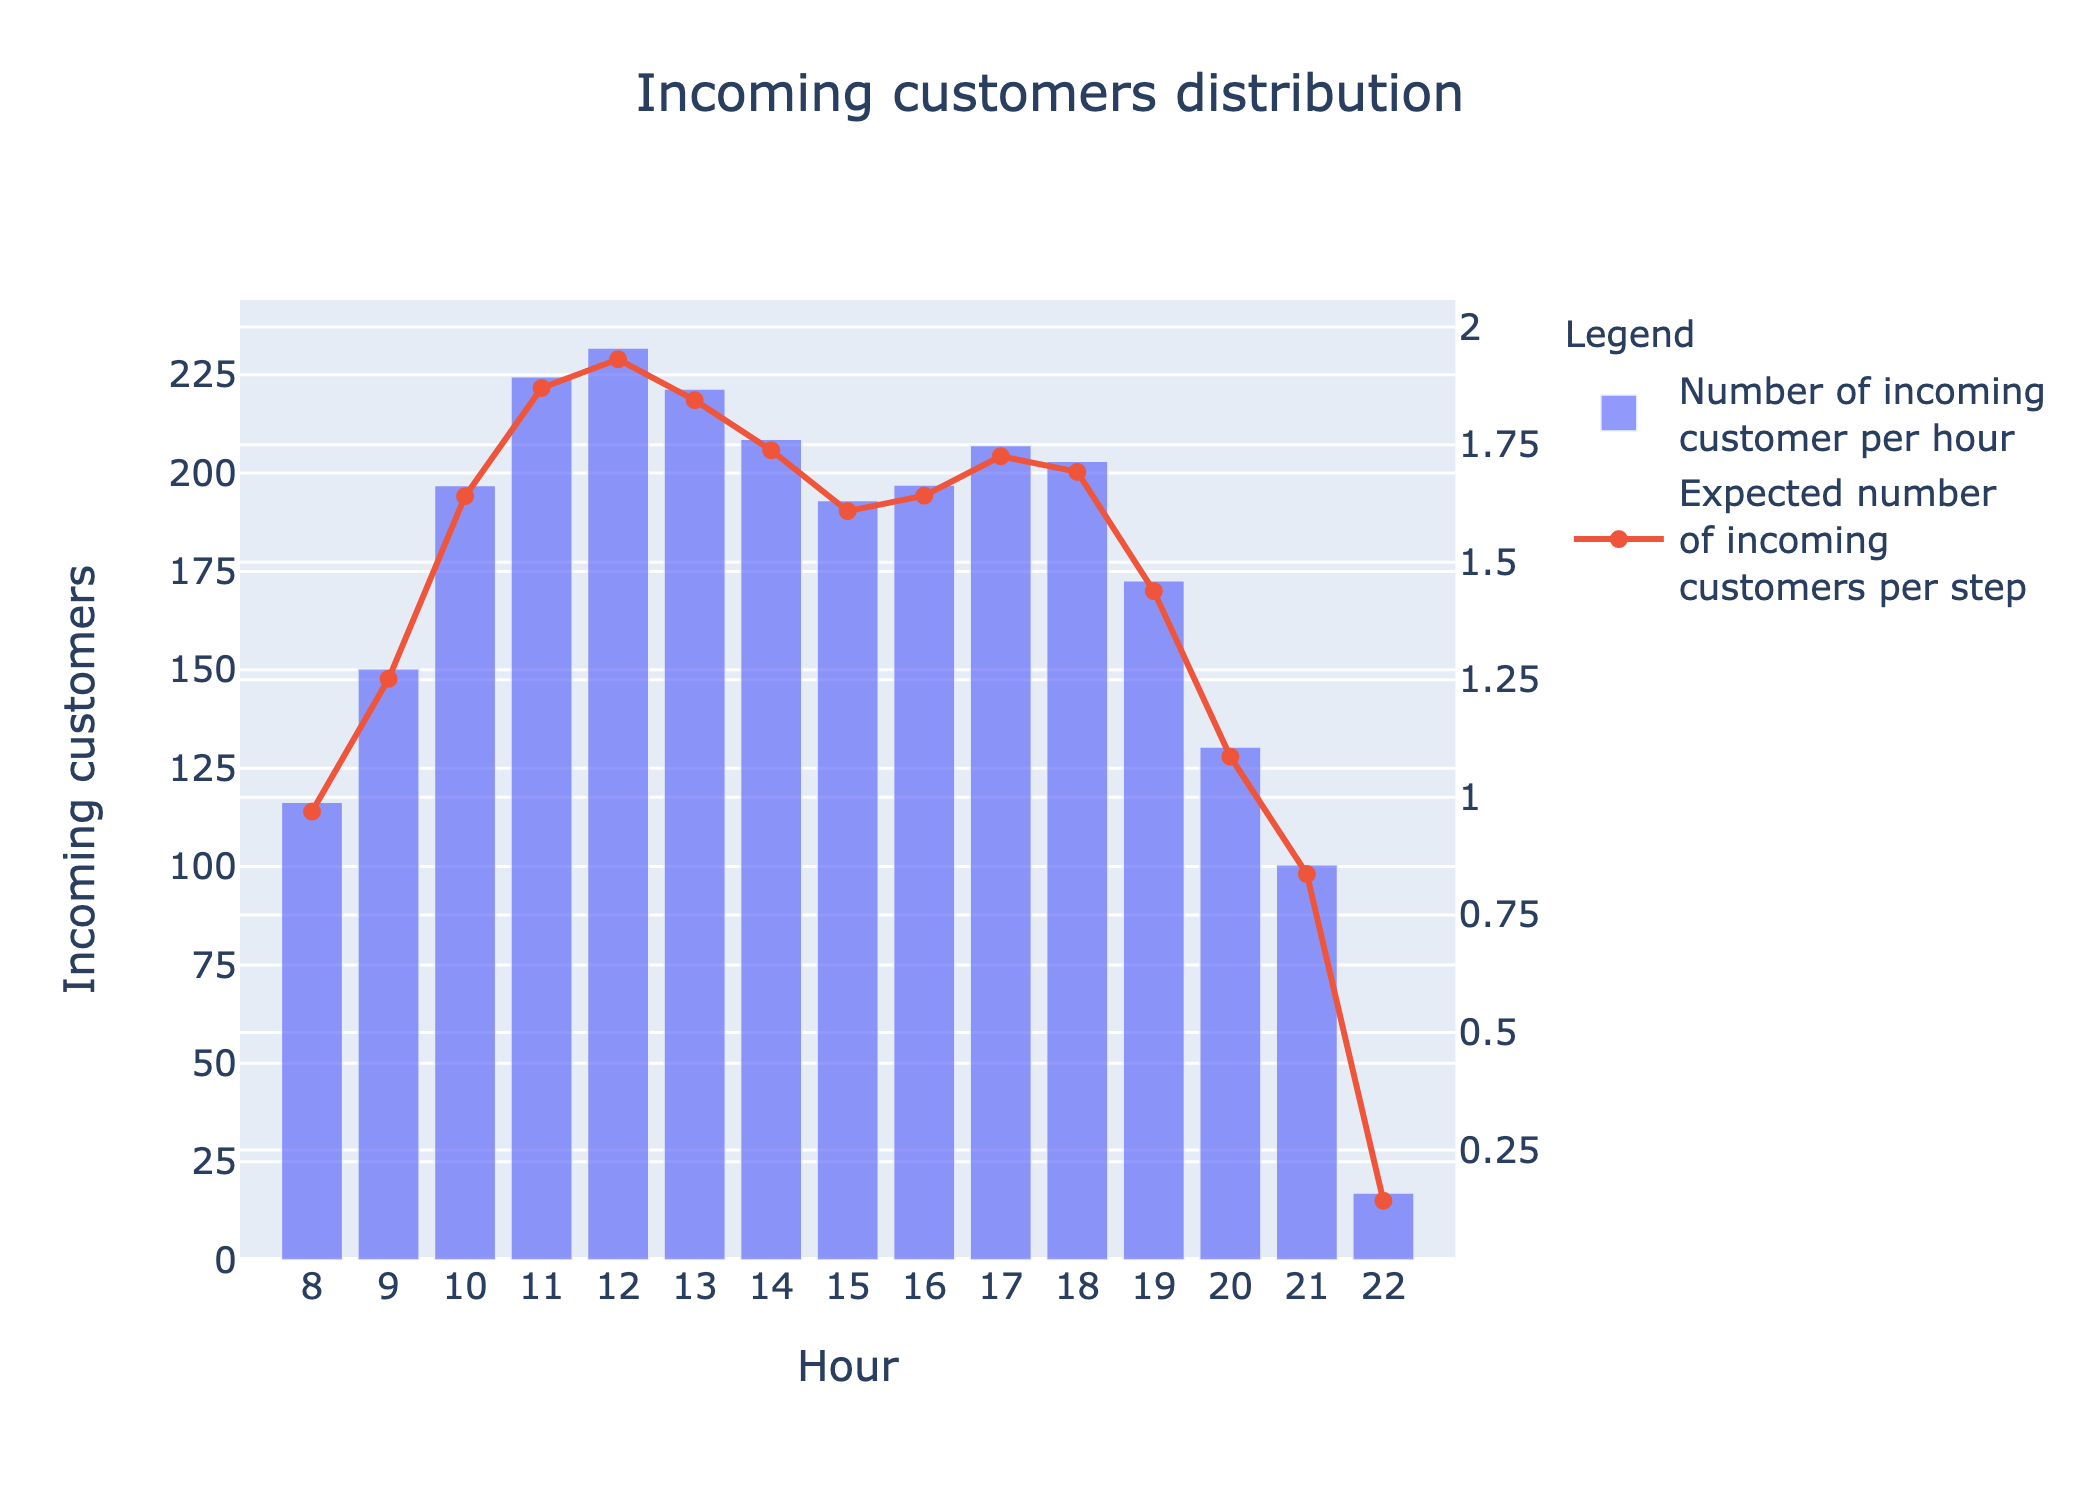
\includegraphics[width=14cm]{"images/per_step_distribution.png"}
	\caption{Valore attesso di clienti in ingresso per ogni step al variare delle ore.}
	\label{fig:per_step_distribution}
\end{figure}

Tuttavia emerge chiaramente come questo valore attesso non sia un valore intero in quanto ottenuto dalla divisione tra numero di clienti totatli in ingresso in un'ora e numero di step per un'ora. Inoltre anche nel caso in cui il valore attesso dei clienti in ingresso per una determinata ora fosse un numero intero, non è realistico che per ogni step di una determinata ora gli ingressi siano identici per ogni step. Per questo motivo si procede aggiungendo del rumore ad ogni step dove il nuovo valore che indica il numero di ingressi per step è frutto della realizzazione della variabile aleatoria $X$ distribuita secondo una normale con media pari al valore atteso del numero di clienti per step e varianza pari a $0.4$. In questo modo si vuole simulare il fatto che ad ogni step possano entrare meno clienti di quelli attessi e viceversa per altri step, pur ottenendo come numero di ingressi totali il valore attesso per quella specifica ora.

Come esempio prendiamo in considerazione le ore 12. In questo orario in media entrano $231$ clieni all'interno del supermercato, vale a dire $1.931$ ingressi per step. Si procede quindi campionando 120 valori (numero di step in un'ora) distribuiti secondo una normale con media $1.931$ e varianza $0.4$. A parire dal valore continuo $x$, si procede discretizzando il numero di clienti in ingresso per ogni step utilizzando la funzione così definita:

\begin{equation}
	f(x)  =
	\begin{cases*}
		0 & se $x\leq0$ \\
		\floor{x + 0.5}       & se $x > 0$
	\end{cases*}
\end{equation}

Nella figura \ref{fig:continuous_vs_discrete_distributions} viene mostrato il risultato dell'operazione di campionamento e discretizzazione.  Alle ore $12$ il numero totale di clienti in ingresso nel supermercato è $231$, si può notare dalla figura che dopo il campionamento e la discretizzazione il numero generato di clienti in ingresso è $232$, che si avvicina molto al valore reale.

\begin{figure}[H]
	\centering
	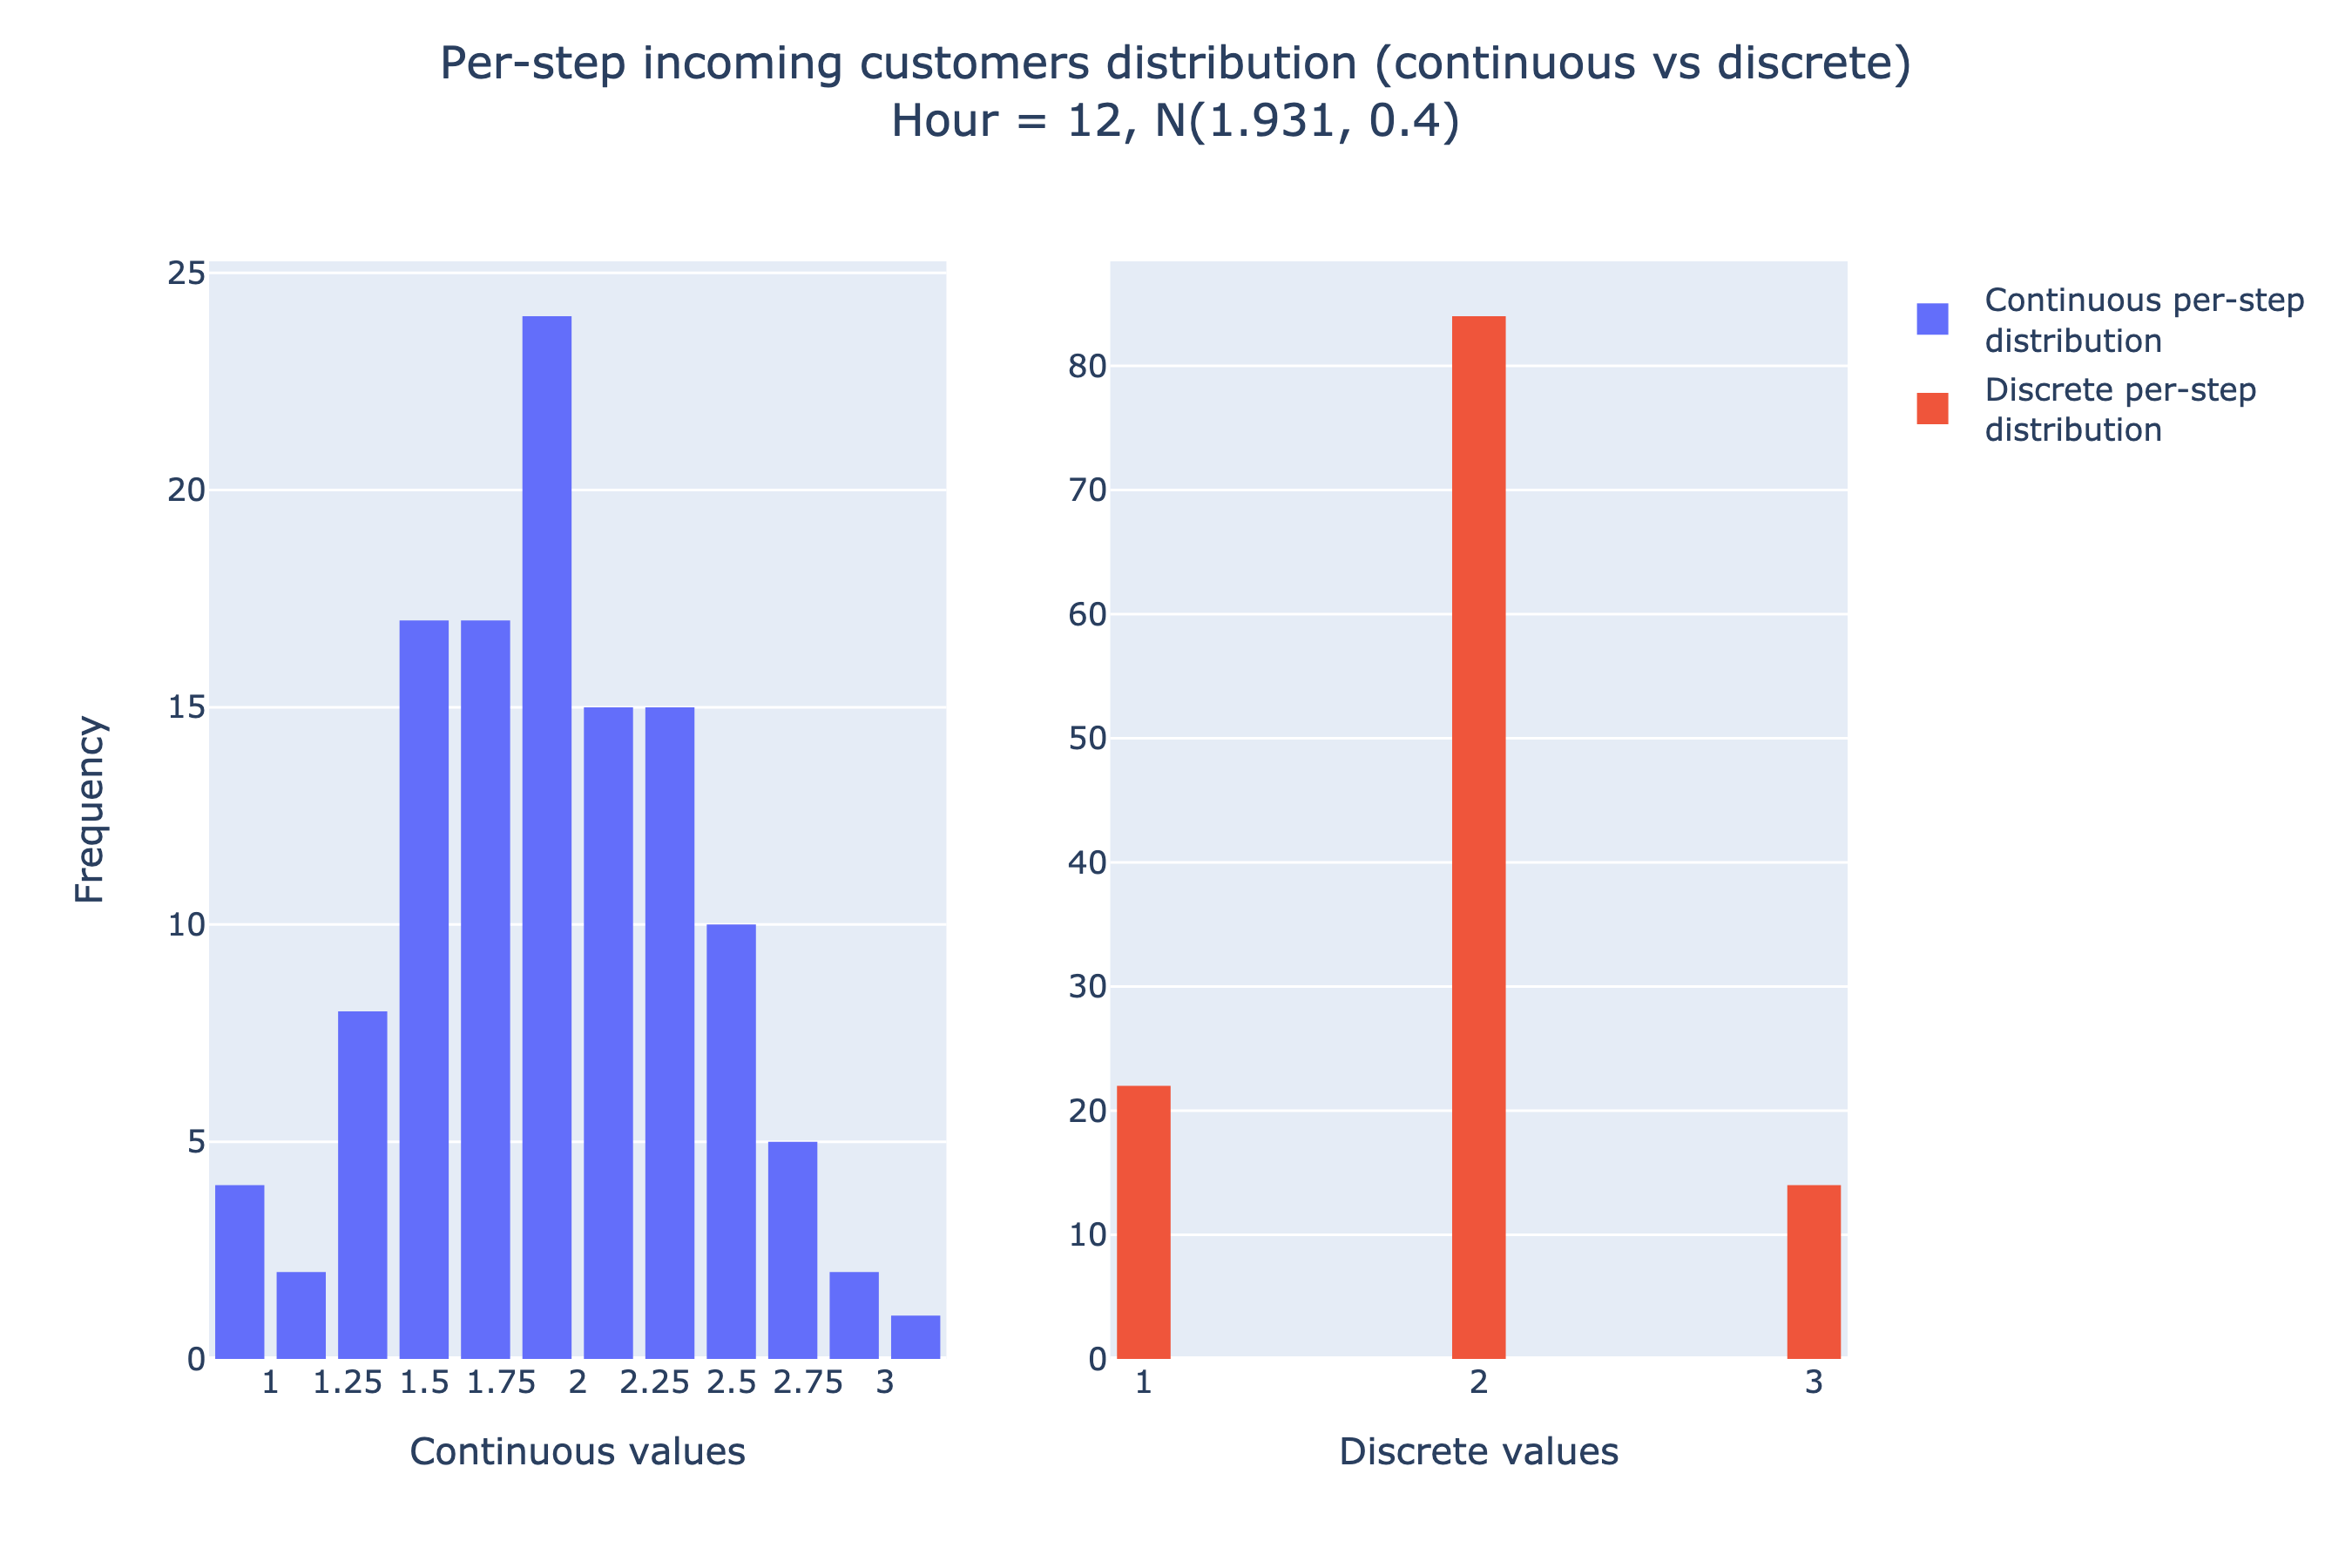
\includegraphics[width=14cm]{"images/continuous_vs_discrete_distributions.png"}
	\caption{Numero di clienti in ingresso per ogni step (distribuzione continua vs discreta).}
	\label{fig:continuous_vs_discrete_distributions}
\end{figure}

Al fine di testare questo metodo che consente di generare il numero di clienti in ingresso per ogni step, vengono eseguiti 30 campionamenti diversi per ogni ora al fine di poter confrontare il risultato con la distribuzione reale. Il confronto tra queste due distribuzioni viene mostrato in figura \ref{fig:real_vs_synthetic_distribution}. Viene inoltre considerato l'errore relativo tra la distribuzione reale e quella generata al variare delle ore. L'errore relativo mostrato in figura \ref{fig:real_vs_synthetic_distribution_error} è ottenuto calcolando: $$Errore = \frac{\abs{X_{reale} - X_{generato}}}{X_{reale}}$$

\begin{figure}[H]
	\centering
	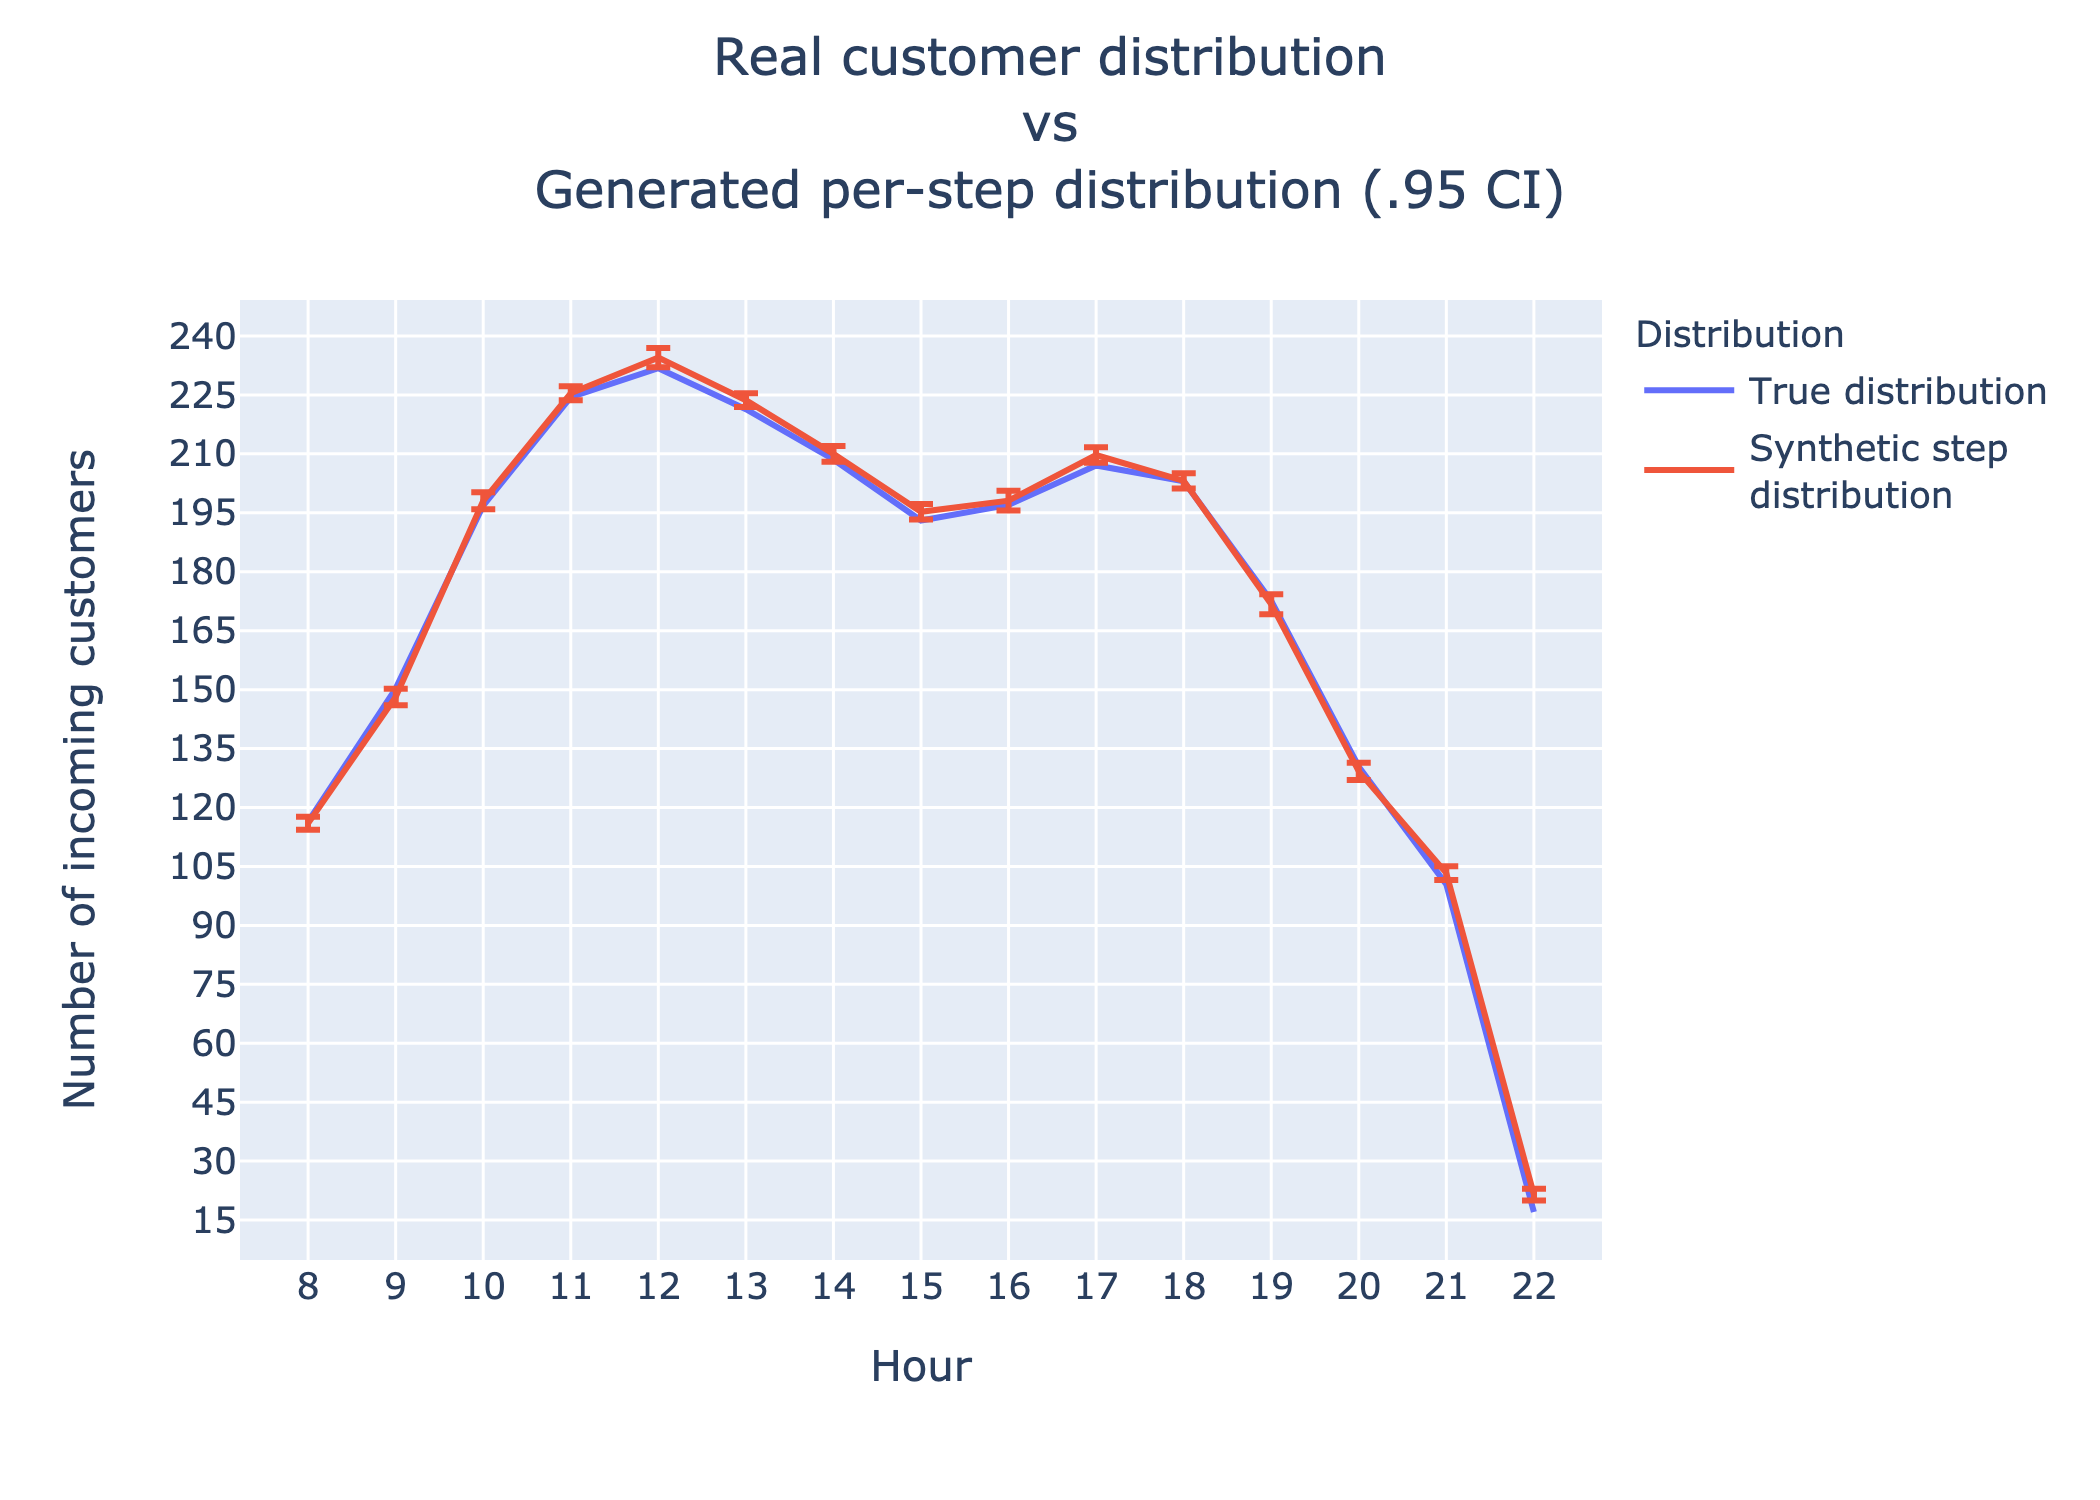
\includegraphics[width=14cm]{"images/real_vs_synthetic_distribution.png"}
	\caption{Distribuzione reale vs distribuzione generata.}
	\label{fig:real_vs_synthetic_distribution}
\end{figure}

\begin{figure}[H]
	\centering
	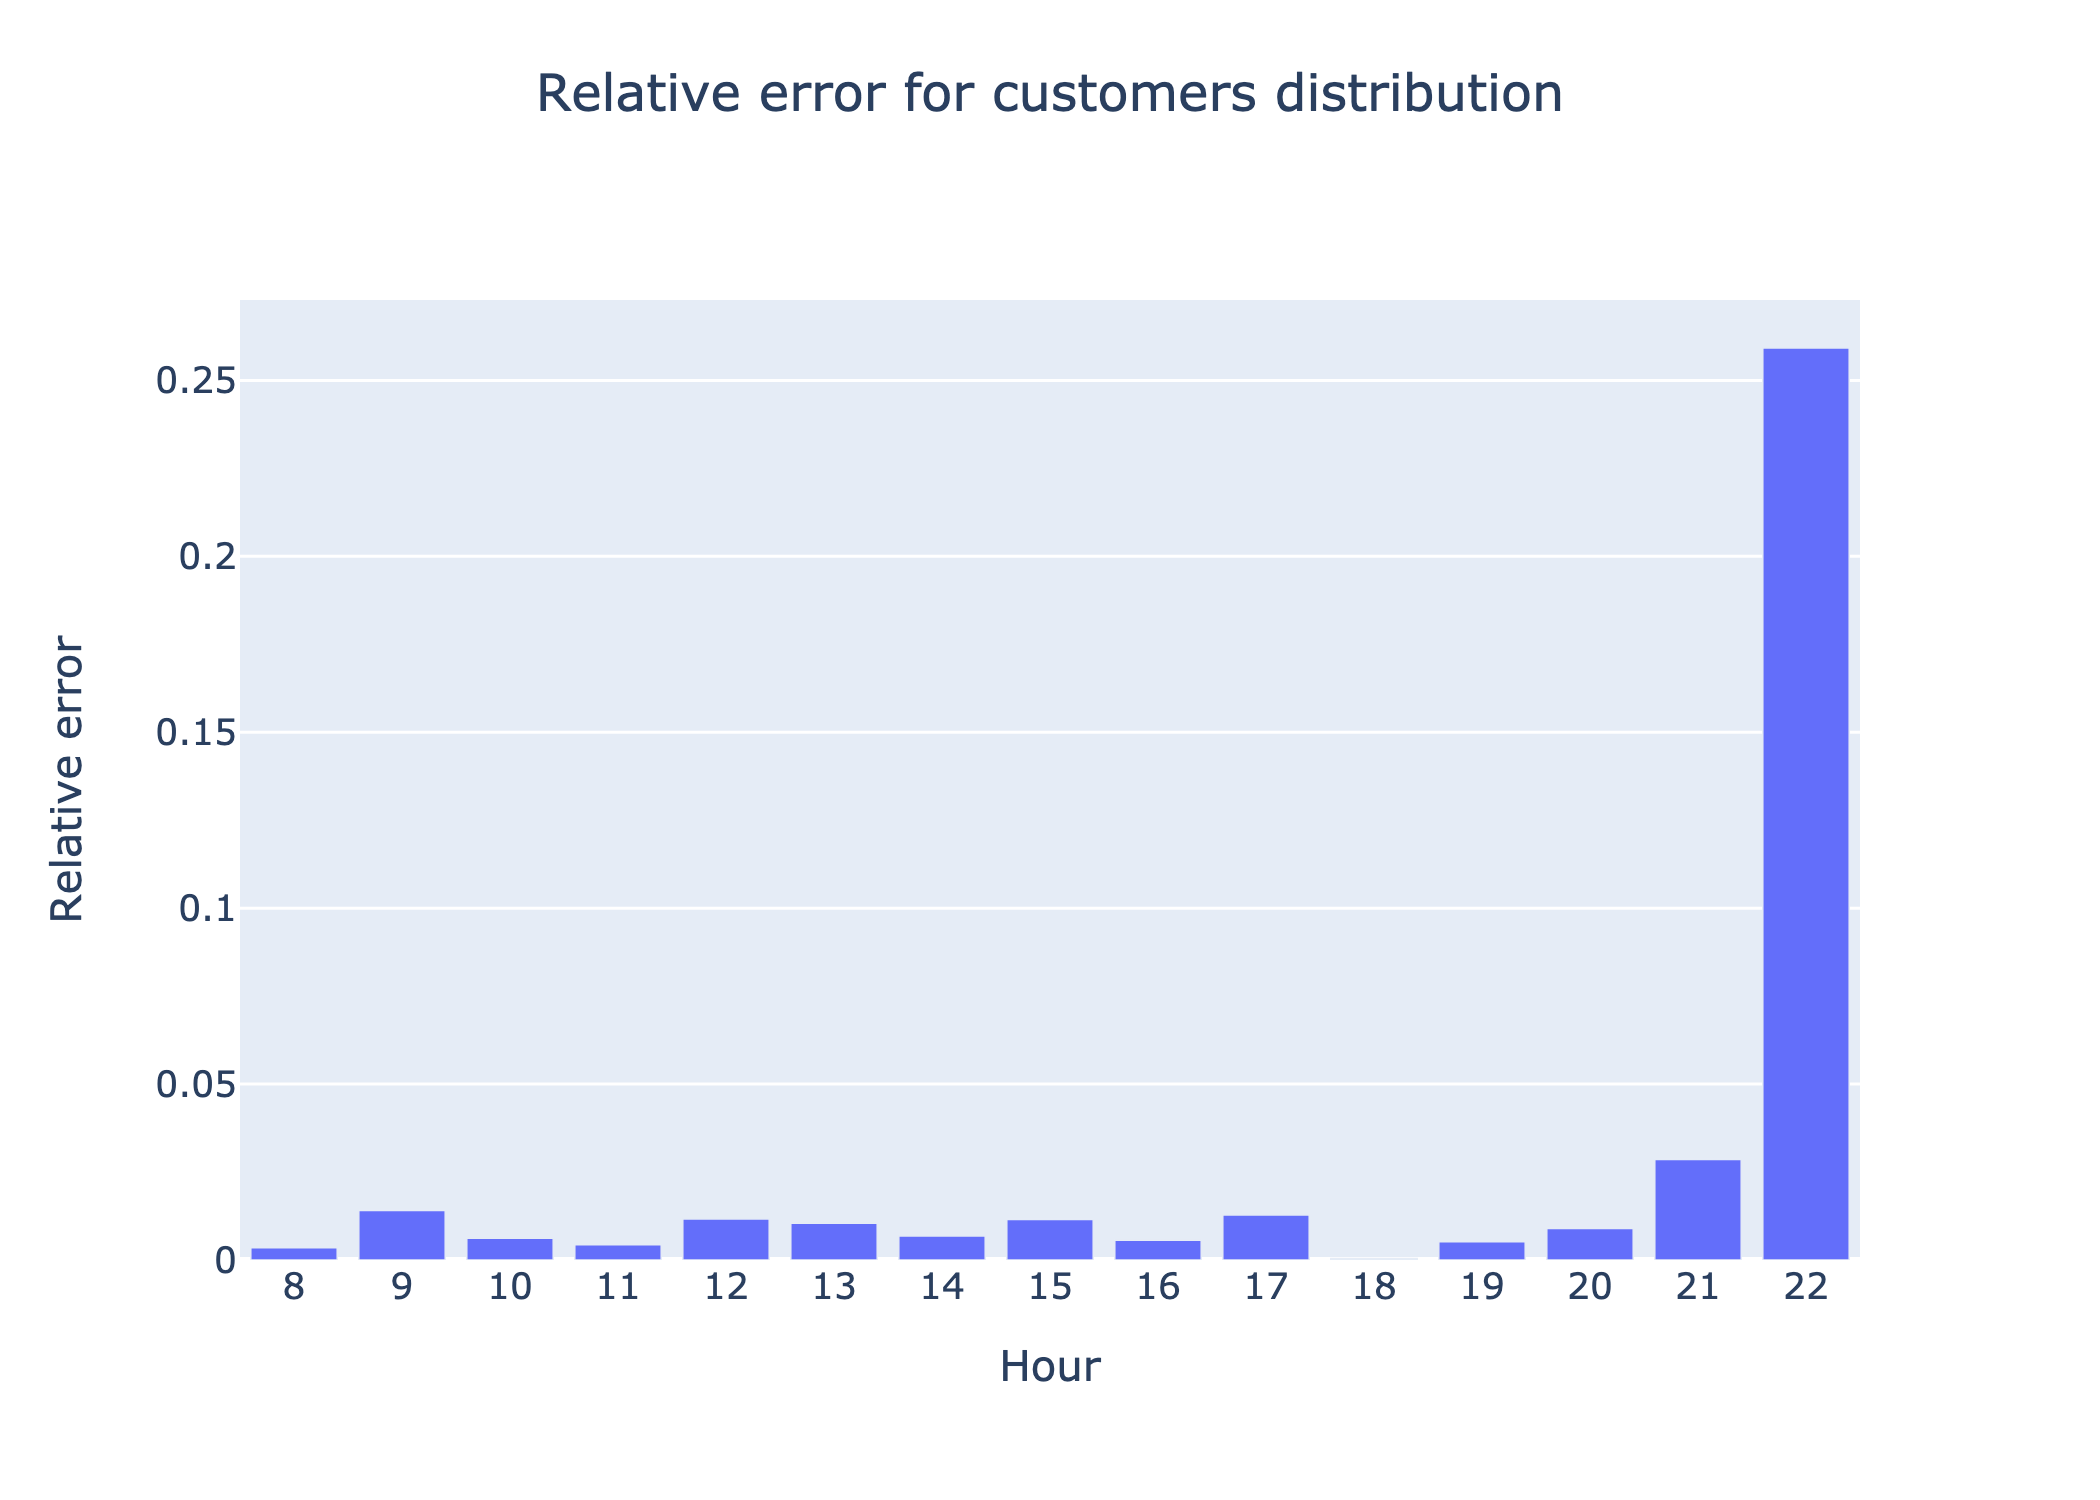
\includegraphics[width=14cm]{"images/real_vs_synthetic_distribution_error.png"}
	\caption{Errore tra distribuzione reale e distribuzione generata.}
	\label{fig:real_vs_synthetic_distribution_error}
\end{figure}

\vspace*{1\baselineskip}

In questo capitolo è stato descritto abbondantemente il modello di supermercato implementato; in particolare si è parlato del workflow e delle capacità degli agenti, oltre che alla flessibilità del modello grazie ai diversi parametri che è necessario specificare per ogni simulazione. Questo ultimo aspetto è un'arma a doppio taglio in quanto molto parametri garantiscono generalizzazione tuttavia portano ad un'esplosione combinatoria delle configurazioni possibili e quindi di difficile tuning in fase di validazione.

Nel capitolo successivo vedremo le strategie di scelta della coda e di jockeying, parte importante della simulazione in quanto l'obiettivo finale del progetto è indagare su quale sia la strategia che minimizza il tempo d'attesa alle casse.